% REMEMBER: You must not plagiarise anything in your report. Be extremely careful.

\documentclass{l4proj}

    
%
% put any additional packages here
%

\begin{document}

%==============================================================================
%% METADATA
\title{3D Animation of Barendregt's Lambda Cube}
\author{Hugo Findlay}
\date{September 25th, 2023}

\maketitle

%==============================================================================
%% ABSTRACT
\begin{abstract}
    The Lambda Cube is a way of visualising how polymorphism, dependent types and type operators combine to form the Calculus of Constructions, where each of the three type systems represents an axis on a Cube.  This theory is often poorly explained, and its digital presence rarely takes full advantage of the medium.  The goal of this project is to help lift the Lambda Cube from obscurity by rendering an interactive 3D version of the cube on a website, to help teach students about the type systems.

    To do this I primarily used the Elm programming language, which is functional, strongly typed and has immutable data.  I conducted user studies using my website to evaluate its performance, and was able to implement the feedback gathered to create a better version of my website.  I believe that this website represents an improvement to the state of information regarding the Lambda Cube and its constituent type systems.
    
\end{abstract}

%==============================================================================

% EDUCATION REUSE CONSENT FORM
% If you consent to your project being shown to future students for educational purposes
% then insert your name and the date below to  sign the education use form that appears in the front of the document. 
% You must explicitly give consent if you wish to do so.
% If you sign, your project may be included in the Hall of Fame if it scores particularly highly.
%
% Please note that you are under no obligation to sign 
% this declaration, but doing so would help future students.
%
\def\consentname {Hugo Findlay} % your full name
\def\consentdate {14 February 2024} % the date you agree
%
\educationalconsent


%==============================================================================
\tableofcontents

%==============================================================================
%% Notes on formatting
%==============================================================================
% The first page, abstract and table of contents are numbered using Roman numerals and are not
% included in the page count. 
%
% From now on pages are numbered
% using Arabic numerals. Therefore, immediately after the first call to \chapter we need the call
% \pagenumbering{arabic} and this should be called once only in the document. 
%
% Do not alter the bibliography style.
%
% The first Chapter should then be on page 1. You are allowed 40 pages for a 40 credit project and 30 pages for a 
% 20 credit report. This includes everything numbered in Arabic numerals (excluding front matter) up
% to but excluding the appendices and bibliography.
%
% You must not alter text size (it is currently 10pt) or alter margins or spacing.
%
%
%==================================================================================================================================
%
% IMPORTANT
% The chapter headings here are **suggestions**. You don't have to follow this model if
% it doesn't fit your project. Every project should have an introduction and conclusion,
% however. 
%
%==================================================================================================================================
\chapter{Introduction}

% reset page numbering. Don't remove this!
\pagenumbering{arabic} 

This chapter talks about the motivation behind the project and its aims.  There then follows an outline of how the rest of the paper is structured.

\section{Motivation}

As of this April 2024, it will have been thirty-three years since the Lambda Cube was first described by Henk Barendregt.  However, it has been an existence marked by obscurity; having little presence on the internet, and rarely being fully depicted.  The motivation of this project was to bring the cube to light and make it easier for students to learn about it.

Lambda Calculus is a computational theory which posits that any computation can be represented by a series of function applications and abstractions.  Lambda calculus has three base units, which construct terms.  These are: Variables, Function Abstractions and function applications \citepp{tapl}.

Simple types are introduced to lambda calculus in order to specify what data is given to a function, and what it outputs. By restricting inputs and defining outputs using simple types, we can make more specific and robust functions.  This is not the only type system that we can add to the untyped lambda calculus, and the Lambda cube is a representation of how three type systems, Polymorphic types, Dependent types and Type operators, combine to form the Calculus of Constructions.

The web format offers the capability to render the cube as a three dimensional experience. This means we are able to show the interconnected nature of the systems which make up the Lambda Cube in a more relatable and dynamic way than a simple paper explanation.  The interactive nature of the website will offer the user to learn by doing rather than just by reading.

There is a difficulty in locating sources about the systems which comprise the cube.  Much of this is because the field of lambda calculus is diverse and old, and interacts with many other fields of mathematics and computing.  A result of this is a wide range of sources, with many using different terminology to describe identical concepts.

There was also a need for a website like this in the University of Glasgow, for the Theory of Computation module, as there are currently few good sources inside the University for this topic.

\section{Aims}

The aims which were identified before the start of the project were: 
\begin{itemize}
    \item
    \textbf{To make learning about the lambda cube more accessible} by giving concise, consistent and relevant information about each system.  To do this I will write about the theory behind each type system as well as explaining the differences in the syntax, beta reduction rules and typing rules in each system or corner of the cube.

    \item
    \textbf{To properly take advantage of the interactivity of the web medium}, as the common explanations around today are mostly in the same format as when the theory was first introduced in the early 1990's.  By allowing the website's user to navigate around a three dimensional representation of the cube, they should be better able to grasp the interconnectedness of the systems, and become more engaged by the learning process by choosing the order in which they learn about the systems.

    \item
    \textbf{To collate useful sources about the systems comprising the lambda cube} as there is not a commonly or easily available list of reliable textbooks or papers about each system.  In order for the website to be a useful educational resource, I will find appropriate and up to date sources for each combination of type systems in the cube, and display them in a clear and consistent manner.
\end{itemize}

\section{Outline}

The remainder of this paper explores and evaluates how I approached these aims, and how successful I was in achieving them.

\begin{itemize}
    \item
    \textbf{Background and Related Work} - focuses on the lambda cube's extant representations online and on paper,  evaluating their merits and considering their weaknesses, learning what ideas can be taken from them.
    \item
    \textbf{Requirements} - talks about the specific  of the website at the start of the project and how they were derived
    \item
    \textbf{Design} - details the research I undertook to select the technology, outlines the architecture and implementation I used, and how I conducted my own research into the Lambda Cube to find appropriate information and sources
    \item
    \textbf{Implementation} - covers the specific implementation used to address each of the requirements, and the issues which arose during the development process
    \item
    \textbf{Evaluation} - discusses the user studies, including details about their structure, results, the actions I took to implement the feedback and how effective the evaluation process was.
    \item
    \textbf{Conclusion} - retrospects the project as a whole and considers how effectively I achieved the aims outlined in the first chapter, and the specific requirements laid out in chapter three.
    
\end{itemize}

%==================================================================================================================================
\chapter{Background and related work}

The untyped lambda calculus was first conceptualised by Alonzo Church in 1932, and is a logical system in which all computations which can be done using a Turing machine can instead be represented by a series of function applications and abstractions.  Another fundamental concept is Beta Reduction, a process which yields a result from an application to a lambda term.  When there are no more possible beta reduction steps, a term is said to be in beta normal form.  Untyped lambda calculus is weakly normalising, which means that not every possible chain of reductions will reach beta normal form.

\section{Typed Lambda Calculus}

The simply typed lambda calculus was introduced in 1940, and allows lambda terms to be constricted to only take certain inputs, and give specified outputs.  Doing this makes the calculus less powerful, but more useful.  Simply typed lambda calculus is strongly normalising, which means that all possible chains of beta reductions will lead to its beta normal form.  The main drawback of simply typed lambda calculus is that its type system is very inexpressive.

Polymorphic types allow you to define terms that are agnostic to their input types, by using an asterisk or star in place of a type.  This allows terms to be generalised, and to depend on other terms, for instance the output type of a polymorphic identity function depends on the term which is input.  This corresponds to System 2/ System F.

An example of a polymorphically typed identity function would be `\texttt{$\lambda \alpha$:*.$\lambda$ x:$\alpha$.x}', where the $*$ stands for any type.

Type operators introduce 'kinds', which are the types of type abstractions.  These let types be defined using other types, and show the structure of type abstractions, but do not contain any information about its content.  These are introduced at the node P\underline{$\omega$} and are generalised using polymorphism in the system P$\omega$.

An example of a type abstraction of a function which takes one type and returns another would be \texttt{$\alpha \longrightarrow \alpha : * $}, showing that it has type kind.  The term \texttt{ $\lambda \alpha : *  . \alpha \longrightarrow \alpha$} would be denoted with \texttt{$* \longrightarrow *$}, because something of type $*$ is both taken in and output.

Dependent types allow you to express types using terms.  This lets you define much more detailed types, however it still has the same computational power, as in the simply typed lambda calculus.  Properties can be encoded into types, which could then checked by a type checker at the compile time of a program, leading to a much safer and more reliable program.  An example of a type depending on the term could be inductively defining a type for all multiples of a given input number.  This type system is introduced at the Lambda-P node.

The three systems combined form the Calculus of Constructions, which is strongly normalising.  This system is mostly used as an aid for formal logic, because of its strong normalisation, forming the basis for the Coq proof assistant.  It can be found at the corner labeled C on the lambda cube show in figure 2.1.

\begin{figure}[h!]
    \centering
    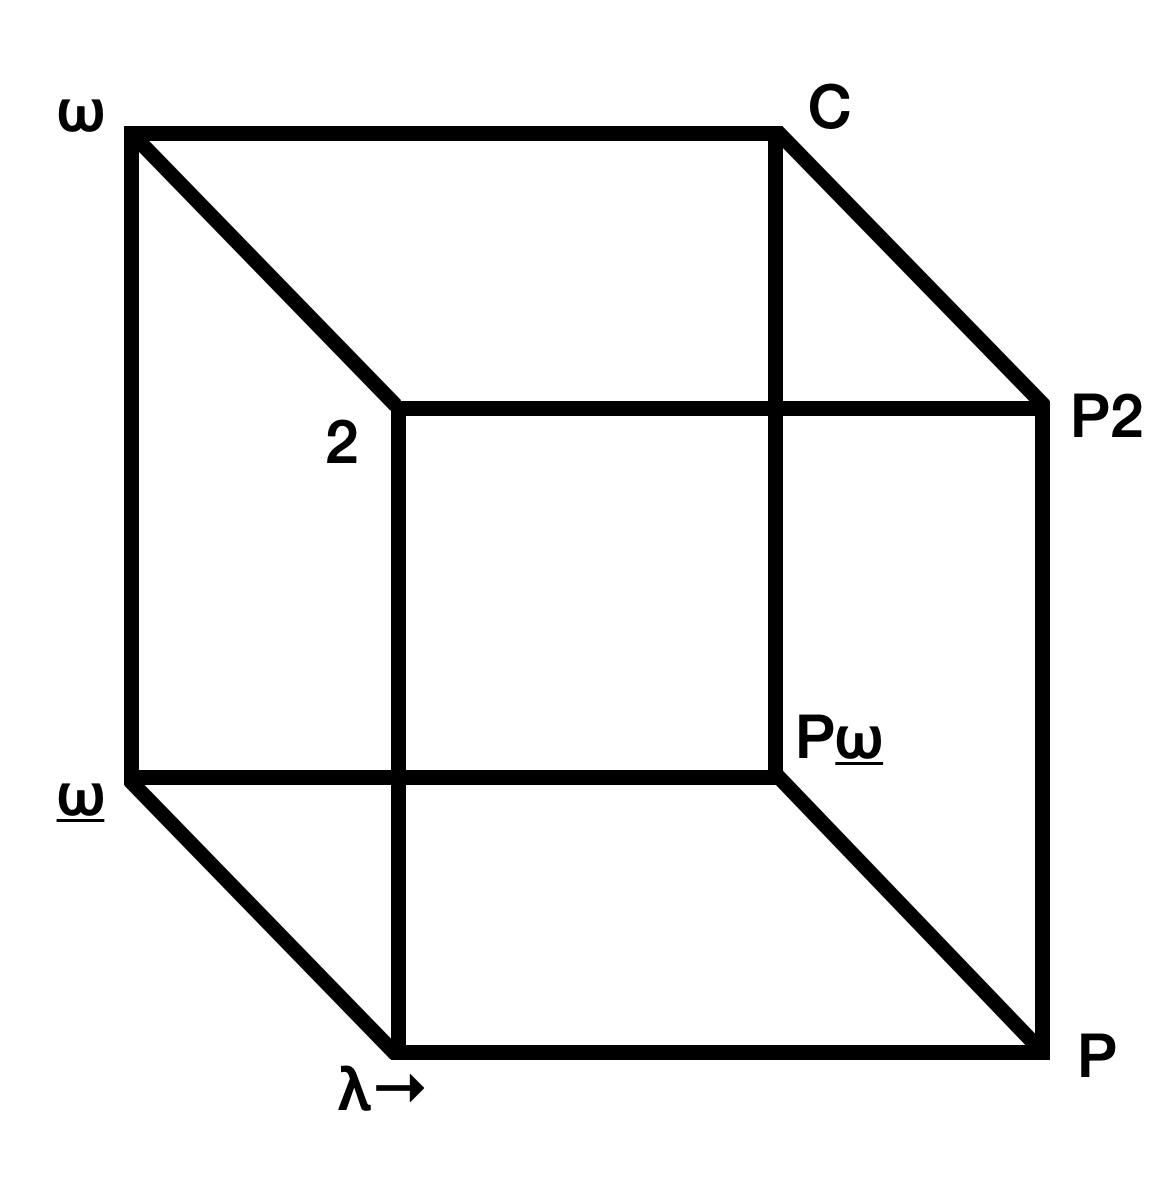
\includegraphics[width=0.5\linewidth]{dissertation/images/cube.png}
    \caption{The Lambda Cube with all of its corners labeled}
    \label{fig:enter-label}
\end{figure}

\section{An Introduction to Generalised Type Systems}
The concept of the lambda cube was first introduced in the 1991 article "an introduction to generalised type systems" in the Journal of Functional Programming by Henk Barendregt \citep{barendregt_introduction_1991}.  The first half of the article explains the lambda cube, and the second half goes on to talk about Propositions as types, the theory that proofs are to propositional logic what types are to programming languages \citep{props_as_types}.  This is related to but distinct from the lambda calculi which my project discusses, and is most linked to the Calculus of Constructions.

As is the first place where the concept of the lambda calculus was introduced, the article has a very good explanation of the way that it is possible for the type systems to interact.  The article includes many proofs and exercises to help explain the concept, as well as using some analogies which to help explain difficult aspects.

For all its achievements, the paper has several notable drawbacks.  Firstly, it is written in a way which is off putting or even inaccessible to people unfamiliar with the topic of lambda calculus, inferring a high degree of knowledge about lambda calculus and formal logic from the user.  It is also plain to look at, written in a standardised academic format.

Due to the nature of this being the progenitor of the concept, and having been published some time ago, there are few sources for some nodes which have since seen further research.  There is also no explanation of the P weak omega system (P\underline{$\omega$}), with the author stating only that he has not been able to find any paper referencing the system.  The Lambda cube itself is also not the main topic of the paper, as suggested by the title, so only half of the already short 31 page count is dedicated to the lambda cube.

\section{Wikipedia}

For many people interested in the topic, the first thing they do will be to read the The Wikipedia page \citep{wikipedia}.  Wikipedia is a website which hosts many articles about a diverse range of topics, with its most important characteristic being that it is a collaborate effort; any user can use their knowledge to improve any page.  With the first iteration of the Lambda Cube page written in 2004 and refactored consistently until 2019, when the page was entirely rewritten.  Since then, the page has remained in a similar state, receiving only minor tweaks and fixes.

This Wikipedia page is written in a way which is much easier for a beginner to understand than the 1991 article, although it has less overall detail and depth to the text.  It also has the benefit of having multiple skilled collaborators, and is able to be updated easily as frequently as needed should new advances be made.  The page also makes liberal use of embedded code fragments to illustrate the application of a type system, where possible.

However, the page is notably lacking in detail about certain critical aspects of each system.  For instance, there is no mention of beta reduction specific to each node.  As well as this, the level of information at each node is hugely variable, ranging between a full paragraph illustrated with code snippets, to just a single sentence.  There are also two systems which are not explained whatsoever, System P\underline{$\omega$} and System P2.  There is also the potential issue of unreliable editors, as the project is open source and freely editable by anybody there is no way to tell if any of the editors are actually qualified.

There is also no explanation of the simply typed lambda calculus on the page, although there are links to it embedded near the start.  As a result of this, new users could become side tracked and end up following only partially relevant links while trying to learn enough background to understand the lambda cube.

\section{The Lambda Cube Unboxed}

The next project I found while researching was a 2021 YouTube series called `The Lambda Cube Unboxed' \citep{youtube}.  Over the course of 13 videos, the creators explain all the concepts required to understand the Calculus of Constructions, starting with Untyped Lambda Calculus.  The series was created by four students and overseen by a professor at the Technical University of Berlin.

This project excels in keeping the user's attention, using interesting and easy to follow visuals and a well written voice over.  The slides are cleanly designed, with an appealing colour scheme and concisely and consistently laid out information.  Additionally, the slides are annotated in time with the narrator's speech, illustrating his point in real time.  This aids in keeping the audience engaged and prevents them getting overwhelmed by the amount of information on the slide at any one time.

\begin{figure}[h!]
    \centering
    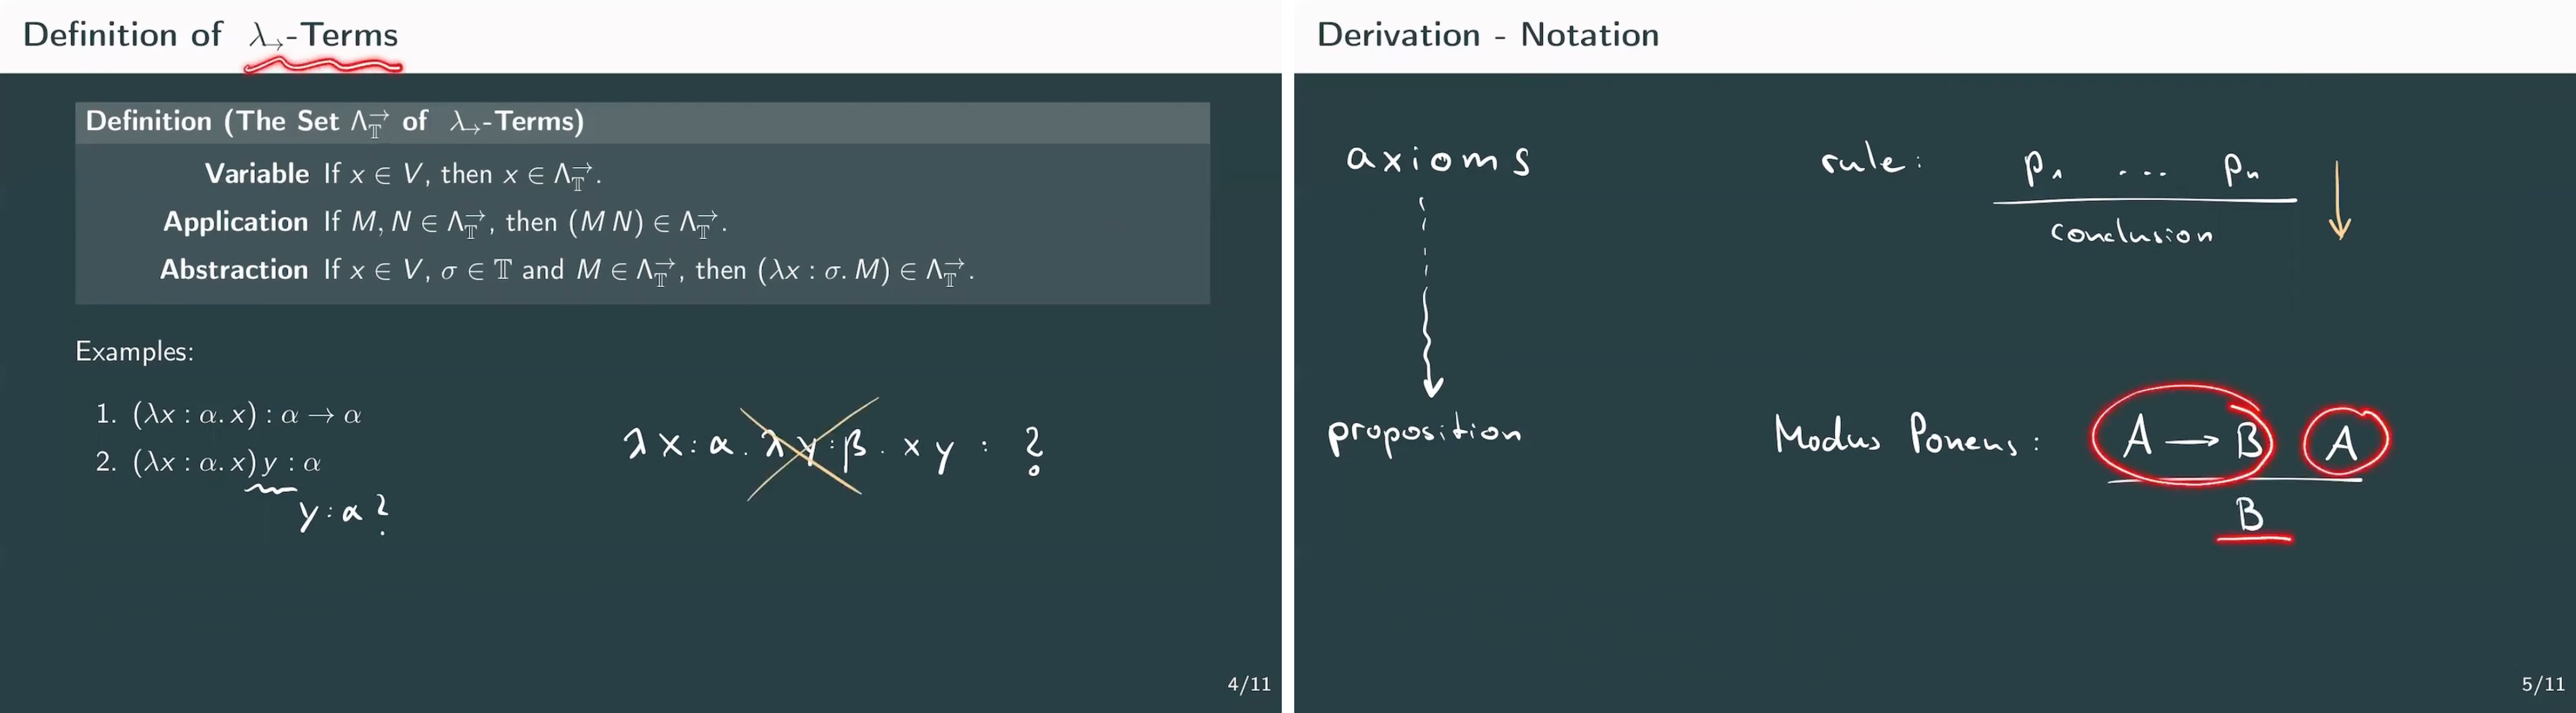
\includegraphics[width=1.0\linewidth]{dissertation/images/unboxed_merged.png}
    \caption{Two example slides from 'The Lambda Cube Unboxed' YouTube series, showing a slide with static information, and one where all of the information is drawn on in real time.}
    \label{fig:enter-label}
\end{figure}

The series falls short in some of the same ways as the Wikipedia page, having few sources and not containing any coverage of the same two systems.  As well as these issues, there were some shortcomings inherent to video, most notably being forced to go at the authors' pace.  As a result, anybody who wants to make notes has to constantly be pausing, rewinding and playing the video in order to not miss anything.  This can be extremely distracting and discouraging to a potential student, as well as boring to listen to the same passage of audio repeatedly.

The medium of video is also not very accommodating to the visually impaired, who cannot use screen readers to receive all of the information that the creator wants them to.  This can be especially damaging to a very diagram or equation rich topic, both of which are relied upon to explain the cube and some of its systems.  A related issue is that there are only automatically generated captions available, likely due to the cost and time associated with manually writing and syncing them to the audio.  Automatically generated captions are generally not very accurate, especially so with rare and precise technical language.  There are numerous parts in the series where the generated captions failed to accurately transcribe the audio.  Consequently the series is difficult to access for hearing impaired students and those who prefer to use subtitles.

\section{Evaluation}

A useful feature common to all three of these representations is the use of equations describing the syntax in a standardised EBNF grammar.  Extended Backus-Naur form grammar is a very high information density medium, and does not have the risk of poor wording misconstruing a fact.  By representing the syntax in a standardised way, it is possible to convey information to anyone who is familiar with the generic syntax language

However, common to all of these projects is the lack of information about the P2 and P weak omega systems, which are sometimes not even mentioned.  There is also the issue of not being thoroughly sourced, making it more difficult for a student to track down additional information about any system that they are interested in.

There are also significant attention reducing factors in each of the works discussed above.  While each is different, there are some commonalities.  The main problem with the 1991 article and 2021 YouTube series was presenting information in a way not instantly and broadly accessible, either because a large amount of prior knowledge was inferred or because the medium does not allow for all of the information on screen at a time.  The Wikipedia page also suffers from this, though not as badly, as it shows the information in a non-standardised way between nodes, and having frequent links to tangentially related pages which can be distracting.

By evaluating the features I liked and disliked from all of the sources I found, I determined that the website would have to be:

\begin{itemize}
    \item \textbf{Independently accessible}, meaning that each node can be understood as much as possible with little prior knowledge of the other sections of the page

    \item The website also needed a \textbf{Consistent Information Layout} so that the user is able to recognise similarities and changes between nodes easily

    \item I also decided that \textbf{Interactive / moving elements} should be used in order to help keep the users attention while presenting dense information
\end{itemize}

By adhering to these principles I would hopefully be able to improve upon previous attempts at explaining the Lambda Cube.
%==================================================================================================================================
\chapter{Requirements}

\section{Problem Specification}
The initial specification for the project mentioned a 3D animation which zooms in on each node, but did not mention the animation to be navigable.  Presenting the information in a pre-determined course and timeline can be a good idea, as it means that you can lay out the information in a logical order, and you will be able to ensure that the user has certain prior knowledge.  However my experience with the videos mentioned in the previous chapter led me to discover the drawbacks of this method of information delivery.

Instead, I decided to make the platform fully user navigable, allowing the user to start and stop at their own pace, as well as start wherever they wanted.  This would have the benefits of affording less experienced users greater time to go through the information, and letting users with advanced knowledge to skip over things that they already know.

\section{User Stories}
In order to gather realistic details about what was needed for the website, I described different ways that potential users could approach the website.  These `user stories' were then refined into specific requirements.

\begin{itemize}
    \item 
        I am a student who wants to get a basic understanding of lambda calculus, but who is not interested learning all of the type systems

    \item
        I am a student who wants to get an understanding of how all of the type systems interact with the simply typed lambda calculus

    \item
        I am a student who wants to get an in depth understanding of some specific systems in the lambda calculus but does not want to learn about every system

    \item
        I am a student who already knows some basic concepts and wants to find further reading materials about the lambda cube
    \item 
        I am a teacher who wants to make my students more engaged with the Theory of Computation using an interactive website
\end{itemize}

By doing this, I was able to find specific and realistic features that I could implement to satisfy the needs of each theoretical user.  Story driven development has the potential benefit of giving realistic and grounded use cases for a website, as well as putting the user's experience first, which is what I planned to do to make the greatest improvement over the previously available explanations of the lambda cube. 

Once the requirements for the project were estimated using user studies, they were prioritised using the 'MoSCoW' technique.  This is when the individual objectives are prioritised into must haves, should haves, could haves and won't haves.  This is beneficial to the software development process because it helps to deliver a minimum viable product swiftly by prioritising only the must haves.  Having a usable website early on in the development process allows for more time to run user studies and implement feedback, as well as making it easier for me to see what areas of the project are lacking than if the website was in an incomplete state.  

It is worth noting that `won't have' goals are elements that would be beneficial to the website but are not in the scope of the current development cycle.

\section{Functional Requirements}

Functional requirements were the exact technical specifications of the website, every function that can be empirically measured.  In my case, this was mainly specifics about what information the website had to contain.  These requirements, as categorised in the MoSCoW system, are as follows:

\textbf{Must-Haves}

\begin{itemize}
    \item There must be a 3D representation of a cube, with each corner or node representing its corresponding point on the lambda cube.  The user must be able to zoom in on these corners by clicking on them, which will reveal more information.

    \item The website needs to host all the information required to learn about the lambda cube.  This needs to include typing rules, beta reduction, an explanation of what makes the node unique.

    \item Each node on the list needs to have a comprehensive list of sources, as without being able to check whether or not a statement is valid, it cannot be considered trustworthy, and the website will be useless as an educational resource.

    \item Accessibility is a top priority.  Using a web platform rather than traditional media gives an often ignored opportunity to make the information more accessible than ever, and there is no reason not to implement these features.
    
\end{itemize}

\textbf{Should-Haves}

\begin{itemize}
    \item It is important that the website experience works on all browsers, and is consistent in presentation between them.
    
    \item The website should also scale to any display or device that it could reasonably be expected to work on.
\end{itemize}

\textbf{Could-Haves}

\begin{itemize}
    \item A night mode would offer greater flexibility in how students are able to use the website, by decreasing discomfort in using the website in dark environments
\end{itemize}

\textbf{Won't-Haves}

\begin{itemize}
    \item A mobile version of the website would theoretically be a nice feature, however the constraints of a much smaller screen and the different input modality of a touch device make the whole design process so different that I would not have sufficient time to do a good job.
\end{itemize}



\section{Non-Functional Requirements}

Opposed to the functional requirements, non-functional requirements are the soft factors of a website.  These are more difficult to define but are equally as important as the functional requirements.  Categorised using the same method as before, these were:

\textbf{Must Haves}

\begin{itemize}
    \item The website must keep engagement better than the Wikipedia page.  As it is the most likely resource people would otherwise use, I decided that it would be a useful benchmark to compare my results to.

    \item The information presented to the user should be as easy as possible for a beginner to understand
\end{itemize}

\textbf{Should Haves}

\begin{itemize}
    \item It should be visually appealing in order to increase the chances that people use it.
    \item The website should have 'replay value', it should be interesting enough to go back to the website across multiple sessions.
\end{itemize}

\textbf{Won't-Haves}

\begin{itemize}
    \item It is outside the scope of the project to add missing information where no research has yet been undertaken, however this is the logical endpoint of the project.
\end{itemize}


%==================================================================================================================================
\chapter{Design}

\section{Animation Framework}

My first idea was to pre-render the animations on my computer and have the website load and play each one when it was required.  I thought that this would make for a well optimised website, as there is little computation going on, with the website simply deciding which pre-downloaded .mp4 file to play at any given moment. 

For this purpose I chose to use the programming language Haskell and the package `reanimate' to create the 3d animations.  I chose Haskell because it is a functional language, and based off of the polymorphic lambda calculus.  It felt fitting for the project to be coded at least partially in a functional language.

I subsequently realised that this approach would lead to very long loading times in low bandwidth situations, which would make the website totally offputting to a lot of potential users.  From a development standpoint it would be more difficult to make small tweaks to, as I would need to re-render the videos each time a change was made, which would be a costly process.  As well as this, it would be more troublesome to scale the video to different resolution screens, without distortion or pixelation associated with stretching or blowing up an .mp4 file.  The combination of these factors led me to decide that I should render the cube and move around it in real time in the browser.

By this time, I had decided to use Elm to host the web portion of my project anyway, so began to search for a 3D web graphic package.  I ended up deciding to use a version of WebGL ported to Elm, as it is able to render both 2D and 3D graphics, and it is also an established technology so has plenty of guides, so would be easier to learn.  GLSL shaders can also be used to render both lines and points, and as GLSL is also a widely used standard there is no difficulty in finding resources or examples.

Although there were other features, I would only need to use the points, lines and camera.  Points were defined as two 3D vectors, one describing its position and the other its colour.  Lines were described as a colour and the start and end points.  Points and lines were both converted into meshes, a type of entity.  These could then be rendered as HTML using a `toHtml' function.  In order to render these meshes, you had to define a virtual camera.  This was constructed of three vectors: an eye (the camera's position), target (the coordinate it should look at) and a vector pointing upwards.  All position vectors are three dimensional, containing the X, Y and Z coordinates.

As I would only need a very simple model to depict the cube, just 12 lines connecting 8 points, it would be incredibly fast and easy to render and re-render the cube continually, the constant animation could be achieved very easily.  I could also use Elm's Model-View-Update structure to navigate between the nodes, as by changing the position of the eye and camera based on the system stored in the state.

\section{Web Framework}

My first instinct was to use Django and Python to host the website, as I had experience with these technologies from the third year team project.  However I soon realised that this was not needed, as it was not necessary to have a back end or database.  Accordingly, I began to research functional web languages, to have internal consistency with my choice of Haskell to generate the animations.  This is when I found Elm.  Elm is a purely functional, strongly typed web language, which draws a lot from Haskell.

Elm runs on a `Model-View-Update' architecture.  This is where the functions which make up the program draws some state from the model, render it as HTML where it is displayed to the user.  The user can then interact with an element, which sends a message that updates the model, changing the HTML displayed.  As all values in Elm are immutable, when changes are made the model is replaced with a new version, with the values that you wanted to change being updated depending on the message.  There are also a large variety of packages available for Elm, which makes it a very versatile tool.

\begin{figure}[h!]
    \centering
    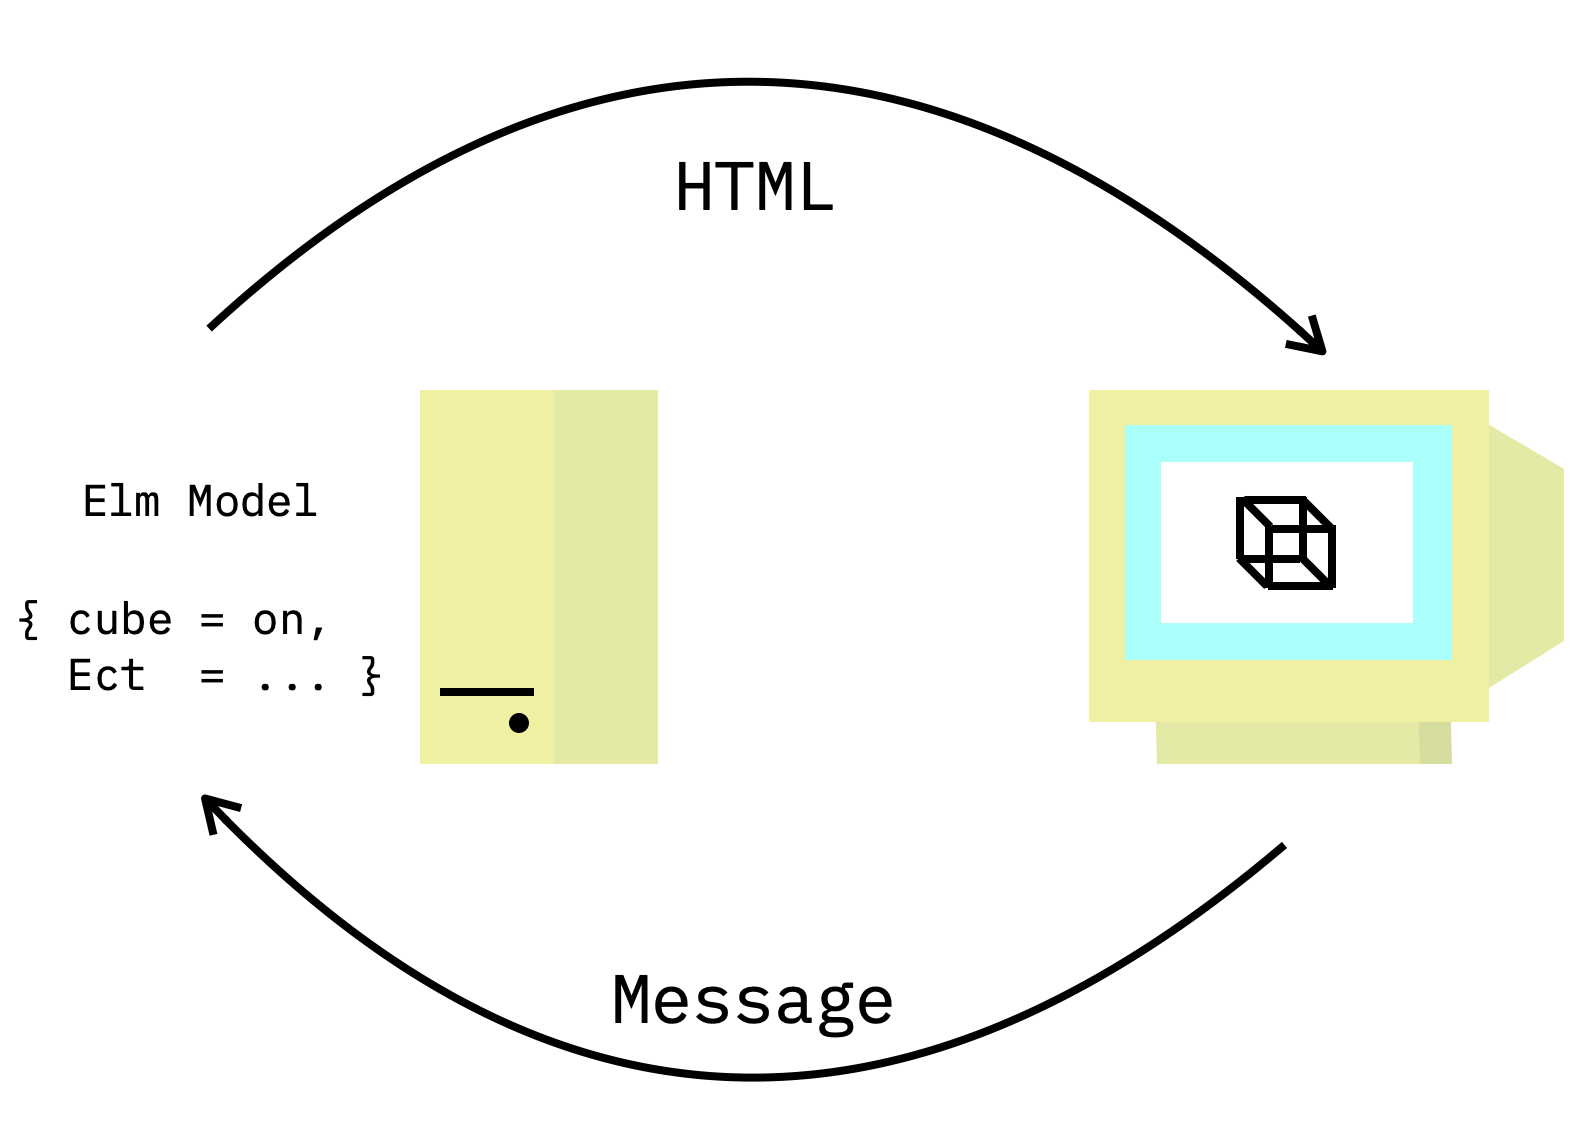
\includegraphics[width=0.8\linewidth]{dissertation/images/elm_loop.png}
    \caption{An explanation of Elm's core operating loop}
    \label{fig:enter-label}
\end{figure}

This concept seemed ideal for my use case, as I planned to have a website that is infrequently updated, and displays a set of pre defined changes whenever there is an update.  In my case, an update to the model would be selecting a different system to view, and the changes I would need to make would be the view of the cube and the information displayed, both of which can be expressed by altering the HTML through changes in the model.

I planned to have as minimal a model and as general message types as possible in order to avoid sprawling repetition heavy code.  Initially, I only stored theta (the time elapsed since the web page was opened) in order to animate the cube, and sys, which would store a custom type with nine options, one for each node on the cube and another for the camera position to show the whole cube at once.

\section{Maths Framework}

There were two main ways of displaying equations on the web that I looked at, these were MathML and KaTeX.  The standard way of displaying equations using a computer is through \LaTeX.  This is a ubiquitous typesetting software which has been in use for over 40 years, and is almost certainly what was used to write the textbooks and papers I was using as research sources.  KaTeX is a library which implements the maths subset of \LaTeX \ into a web format using JavaScript.

MathML is a better choice for displaying mathematics, as it is more compatible with screen readers such as MathPlayer, which is incredibly important for accessibility reasons.  For this reason, I initially tried to write all of the syntax out by hand in MathML.  This is a mistake, as the language is incredibly complex and tedious, with complex equations such as I needed requiring many nested layers, making it easy to make mistakes.  Because of this, I quickly abandoned this approach.

I subsequently found that was an existing library which ports KaTeX to Elm.  However, upon trying out this library, I was disappointed with its results.  There was a noticeable lag between when an element containing KaTeX was displayed, and when the content inside it would compile into HTML and load.  The pop-in effect made the website seem amateurish and untrustworthy, so the package was not suitable.  Additionally, the way the library expected code to be written was far more complex than it needed to be.

It is at this point that I decided that there were currently no solutions to my problem, so determined that I would have to write my own program to translate .tex files into Elm.  By doing this, I could have much more granular control over how the KaTeX was displayed, and would be able to pre-compile all of the equations that I needed, which would avoid the pop-in issue.

I used the Deno runtime for JavaScript to build my translator because it was advertised as low overhead, so I hoped that it would be minimally invasive to add to my technology stack midway through my project.  In specific I used the Deno DomParser to read HTML rendered by KaTeX. 

I found Deno to be very easy to work with, and never found it to be lacking in functions which I wanted to use, although I did use it only for one specific purpose.  There are plenty of other technologies that I could have used, such as Bun or Node.js.

\section{Site prototyping}

I decided very early on to use colour heavily in the design of the website.  By using red green and blue to represent the Dependent types, Polymorphic types and type operators specifically, I could intuitively show how the systems merge by mixing the colours.  For instance, if you have Polymorphic types and type operators, then blue and green mix to form teal, so teal is used at that node, if you used both dependent types and type operators, you would have purple.  This system should also build up recognition of the different type systems faster, by being able to associate the type rules with both a name, axis and colour.

One significant problem I realised I would have is that when zoomed in at a node, different parts of the screen are taken up by the cube each time.  This was an issue because it meant that the information would either have to change layout at every single node, resulting in an inconsistent and confusing website to use, or leave the information in the same place and occlude parts of the cube.  I decided that it was more damaging to the experience to block out parts of the cube than to move the text boxes around, and to ameliorate the issues caused by this I would give three different text box types (syntax, explanation and beta reduction) distinct styles so that the user always knew where to look for specific information.

The first designs of my website were done on paper, as it is easier to quickly prototype different designs.  The final version I sketched on paper can be seen beneath.

\begin{figure}[h!]
    \centering
    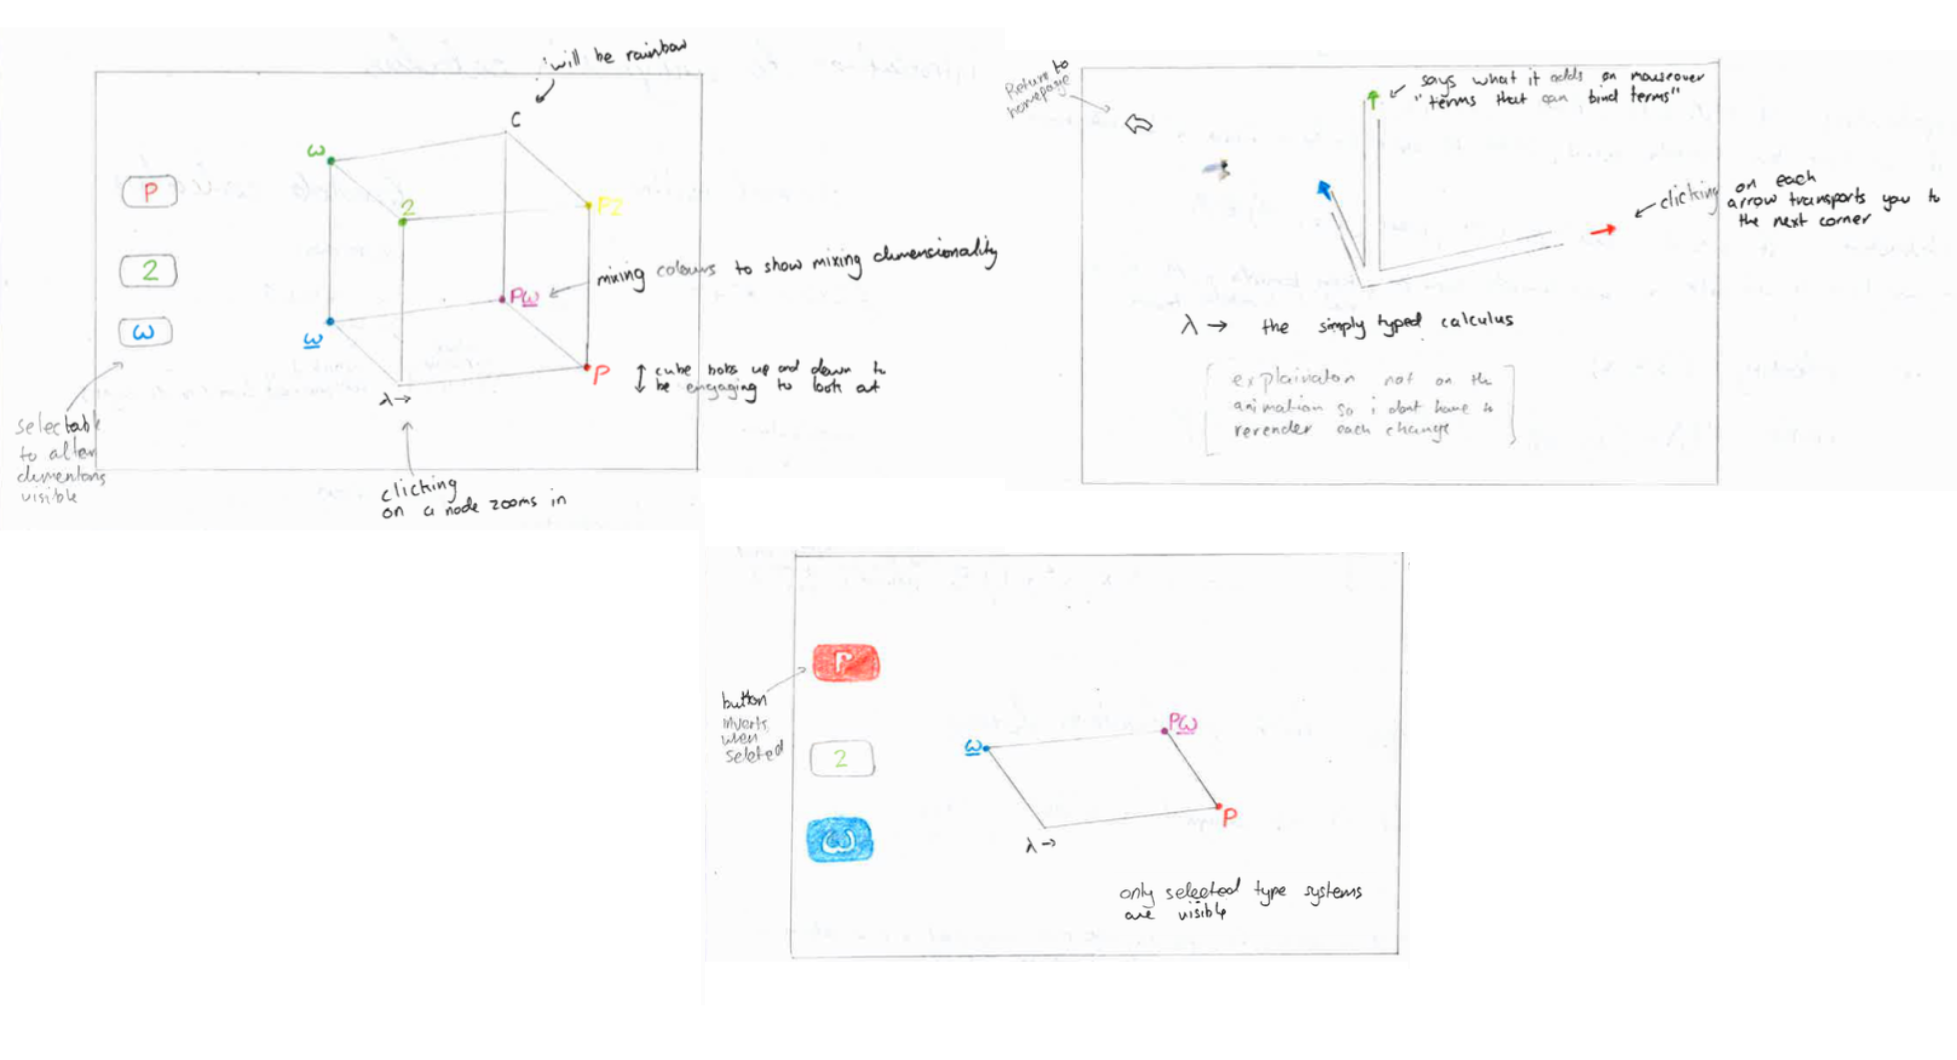
\includegraphics[width=1\linewidth]{dissertation/images/paper_collaged_taller.png}
    \caption{A scan of my final paper sketch ideas}
    \label{fig:enter-label}
\end{figure}

The (collaged) scan shows the three main states that I planned for my website to have.  The top left shows the home page in the normal state when the website has just been opened.  This has a diagram of the cube, with the corners labeled in the colours derived by mixing those I assigned to the axes.  I also included notes that the cube should constantly be moving slightly.  I decided to do this so that the page would not look as boring and static, which would hopefully aid in keeping the user's attention.  

There are three buttons on the left side of the screen.  I planned to have these as a way of removing type systems from the cube, so that there would be only a line or square if one or two buttons were selected respectively.  This could be used to narrow down the amount of information presented on the screen at any one time, to avoid overwhelming a new user by narrowing down the potential options available to them.  This would also let an experienced user refine their use to only show relevant information.

After this, I transitioned to using Figma to further develop my design.  I chose to use Figma because I was already familiar with the technology from the third year team project.  Figma is better to use at this stage of the project as it allows you to undo and redo actions, as well as copy and paste similar elements, which cannot be done with pen and paper.

\begin{figure}[h!]
    \centering
    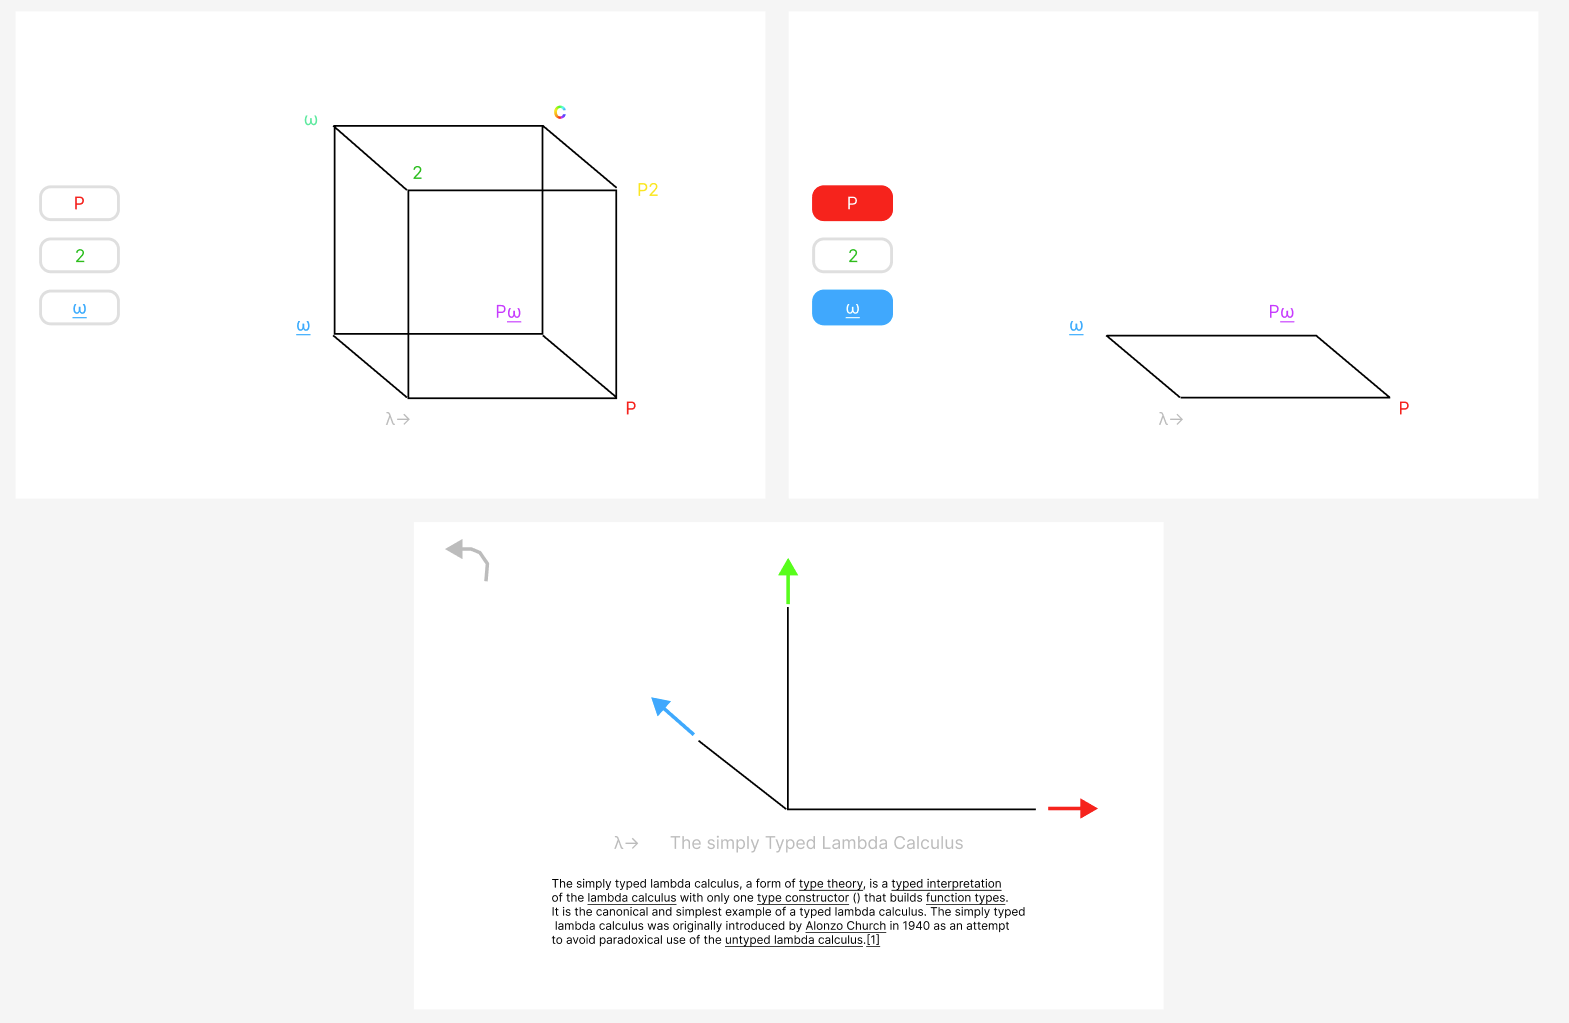
\includegraphics[width=1\linewidth]{dissertation/images/v1_full_taller.png}
    \caption{A screenshot of the first Figma version}
    \label{fig:enter-label}
\end{figure}

While refining my design in Figma, I decided to delete the function to show and hide dimensions, as it did not seem useful.  I concluded that it did not offer more functionality than clicking on a single node, or just looking at one dimension at a time using the arrows.  As well as this, it could be seen as confusing to some users, who might not understand the concept or could remove a dimension and forget to re add it later, potentially locking them out of learning more.

I repurposed the side button elements into buttons which allow the user to move to a different node instead.  I also decided to put the page contents into text boxes that I would position around the screen, instead of being in one scrollable section in the middle.  I chose to make this change after having to constantly scroll up and down in papers to read different sections, and noticed that this could be largely eliminated by making better use of the empty space in and around the cube.

\begin{figure}[h!]
    \centering
    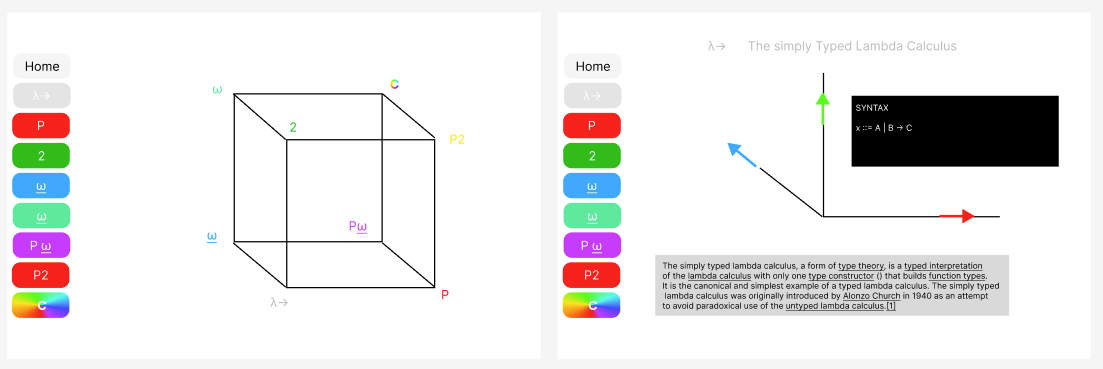
\includegraphics[width=1\linewidth]{dissertation/images/v2_full.png}
    \caption{A screenshot of the final Figma version}
    \label{fig:enter-label}
\end{figure}

While writing the explanations for the type systems, I realised that the website would be incomplete as a tool without an explanation of untyped lambda calculus.  This presented a problem for the design, as there is no spot on the cube which represents the untyped lambda calculus.  The way which I addressed this was to add a separate point to my WebGL model which is not in view from home, but is accessible using the sidebar.  This shows a clear distinction between the typed and untyped calculi, while still having an easily accessible explanation of the basics of untyped lambda calculus.

I chose to use IBM Plex sans as the main typeface for my website.  I made this decision as it is a modern, recently released font, which lends a feeling of novelty and credibility to the site.  The University Style Guide also recommends using sans serif fonts as far as possible, as they are easier to read than more complex, serifed fonts.  I chose to use a medium font weight, as it would stand out more on small screen and in low contrast situations, while being more dense than a bolder font weight which would take more space to display the same amount of text.

Another benefit to using this particular typeface is its near comprehensive Unicode support.  Much of the content on the website relies on characters which are not present in a lot of fonts, specifically Greek letters such as $\lambda$ or $\omega$.  As there are versions of these characters inbuilt, they can be displayed in a more cohesive way than if I was using a typeface without support for these characters.  There are versions of the font available in all major scripts so in future the website could be translated into other languages without having a significant disruption in style.  It is also open source, meaning that it is free to use without a licence.  This makes it more suitable to be used by the University in an official context, as they would not need to spend departmental resources on a font licence.

\section{Research}

As I had only a small amount of prior knowledge, and had not received any lessons about lambda calculus at the beginning of my project, I knew that I would have to spend a significant amount of time researching the different type systems and the way that they interact in order to be able to write acceptable summaries for each node.

Although some of my background research doubled as research into the systems which made up the lambda calculus, I still had to learn a significant amount more about every single system in specific, both to be able to write the summaries and validate the usefulness of currently available solutions.

Researching each system enough to be able to write the content for each node proved to be greatest struggle I had during the design phase of my project.  In chapter two of the original article from 1991, Barendregt lists each system of the cube and mentions the most significant research which has been done about them.  Most of these references are descriptive and were very helpful to find further sources, however the only note about system $\lambda$ P2 is that "[it] is studied by Longo and Moggi (1988) under the same name", and system P\underline{$\omega$} "seems not to have been studied before".

P\underline{$\omega$} was incredibly difficult to search for, as I struggled to believe that the system had truly remained unresearched in the over thirty years since it was described in the paper.  It was also never described in more than the vaguest details in works such as the Wikipedia page or Lambda cube unboxed, with these sources just gesturing towards its existence in graphs of the complete cube.  

Searching for P2 was also very difficult.  The only reference which I found was to the 1988 paper by Longo and Moggi, which proved tricky to track down as it is titled "Constructive natural deduction and its ”omega-set” interpretation", which is easily confused for the system Omega.  Once I found it it was not especially useful, lacking certain specific details which I needed, such as a comprehensive BNF or EBNF style syntax for the system.

Google searches for both of these systems returned zero useful results, only a few descriptions of the lambda cube as a whole where the corners were labeled but never explained at all.  Both when using the term P2 or Second order predicate calculus, there were few results.  Some searches for system P2 resulted in sources for system F, and searching for system P\underline{$\omega$}

Eventually, I posted a question onto the Theoretical Computer Science Stack Exchange, asking if any users there were familiar with any works which mention system P\underline{$\omega$} in depth. This is a website where users can ask and answer each other's questions specifically about theoretical computer science.  Although there is no verification process to ensure the qualification of an answer, each user is given a reputation score, which is increased by having their answers highly rated.  

My concerns about the validity of responses was also diminished, as I was asking about sources, and not specific details, about the two systems, so I would inherently be getting an answer whose validity would be easy to check, simply by reading the paper suggested to see if it is relevant.  My question eventually received an answer, and using that I was able to verify that there has been no further research into P\underline{$\omega$}, as well as find a more modern and relevant paper regarding system P2.


%==================================================================================================================================
\chapter{Implementation}

Before starting this project, I had never used Elm or created a website on this scale alone.  The first part of the code that I worked on was the cube animation, as the rest of the website is defined in relation to the cube, making it the logical place to start.

\section{Using Elm}

The core of an Elm program is its model.  TODO DEFINE MODEL.  In the design phase I planned to have an incredibly slim model and to derive all of the state from the system variable.  However after implementing more and more features, the complexity of the model increased in size to have ten entries.  The final version of my model, including the refinements made after the user studies, is shown beneath.

\begin{lstlisting}
type alias Model =
    { theta : Float
    , system : System
    , target : Vec3
    , eye : Vec3
    , banner : Bool
    , footer : Footer
    , syntax : Bool
    , reducedMotion : Bool
    , theme : Theme }
\end{lstlisting}

The fields I had in the model were:
\begin{itemize}
    \item \textbf{theta}, which had the type Float.  This keeps track of the time since the website was loaded, and is used to make the cube rotate.

    \item \textbf{system} is the most important part of the model.  It is used to position the camera and change what was displayed in the syntax boxes.  This has the type `System', which is defined as: 

    \begin{lstlisting}
        type System
            = Home | None | Simple | P | Two | W_ | W | PW_ | P2 | C
    \end{lstlisting}
    Each point has a value corresponding to each point on the cube, as well as `Home' which shows the whole cube at once and `None' which is used to explain the Untyped lambda calculus.

    \item \textbf{target} is a 3D vector which has an X, Y and Z component, each of which is a float.  This value is used to determine the point where the camera is looking

    \item \textbf{eye} is also a 3D vector, but is used to define the position of the camera

    \item \textbf{banner} is a boolean value which is used to determine if the references panel should be shown or not

    \item \textbf{footer} is used in a similar way to banner, and is set to a custom type, Footer, which has the signature
    
    \begin{lstlisting}
        type Footer
            = Closed | Settings | Guide
    \end{lstlisting}

    As the settings and guide panels are very similar elements, I decided to have them be variants of the same element,  sharing the same shell code with the value footer determining what was stored inside, or if footer was set to `Closed' then it would be hidden.

    \item \textbf{syntax} uses a boolean to decide which version of the syntax box to show to the user

    \item \textbf{reducedMotion} takes a boolean from a CSS variable set when the website first loads.  This boolean is then used inside the animation, where a true value will stop the cube from moving.

    \item \textbf{theme} is another custom type, which has two variants.  These are used to decide if the website should be using the safe colours or not.  This value is also set from a CSS variable when the page loads

    \begin{lstlisting}
        type Theme
            = Normal
            | Colorblind

    \end{lstlisting}
\end{itemize}

The addition of target and eye was to facilitate the linear interpolation of the camera position.  Reduced motion and theme were added to enable the accessibility features implemented after the user study.

Messages to update the model are another critical part of the Elm structure. These determine how the model is updated and to what value.  I ended up with seven messages in the final version of my website, which are listed beneath.

\begin{lstlisting}
type Msg
    = Tick Float
    | SystemClicked System
    | ToggleReference
    | FooterClicked Footer
    | SetSyntax Bool
    | ToggleReducedMotion
    | ToggleTheme
\end{lstlisting}

\begin{itemize}
    \item \textbf{Tick} takes a float from the subscription, and uses it to update the value of Tick in the model.  It is the only message to not be sent using an OnClick event.

    \item \textbf{SystemClicked} is used as the OnClick property for the corners of the cube, the guide arrows and the arrows on the edges on the cube.  It takes a value of type System and sets the value of system in the model to its argument.

    \item \textbf{ToggleReference} is used to show and hide the element which has the references for each node.  It does this by flipping the boolean `banner' in the model.  All it needs to do is change a boolean from true to false or false to true, therefore the message does not need to take an argument.

    \item \textbf{FooterClicked} takes a custom type Footer, and updates the footer field in the model.

    \item \textbf{SetSyntax} takes a boolean value and sets syntax to this value in the model.  This is used to control which tab is shown on the syntax box.  We cannot just invert the value, as then clicking on the same tab twice would have no effect.  This is not how the same system works in a web browser, so the system should follow the paradigm that the user is probably already familiar with.

    \item \textbf{ToggleReducedMotion} toggles the boolean value reducedMotion in the model, and uses the port setReducedMotion to update the reduced-motion value in local storage.

    \item \textbf{ToggleTheme} updates the theme variable in the model, and uses the port setTheme to update the prefers-high-contrast value in local storage.  Because the value in local storage does not have the custom type `Theme', I had to use a let binding to get the new value from the current state of the model, and then call a helper function to convert theme into a String before it is sent, as follows:

    \begin{lstlisting}
        ToggleTheme ->
            let
                newtheme =
                    if model.theme == Normal then
                        Colorblind

                    else
                        Normal
            in
            ( { model
                | theme = newtheme
              }
            , setTheme
                (Context.theme2string newtheme)
            )
    \end{lstlisting}
\end{itemize}

An example of a message which I used a lot was \texttt{SystemClicked}.  This was how I moved the camera between different nodes and decided what content would be shown at each node.  The code for the message was as follows.

\begin{lstlisting}
SystemClicked sys ->
    ( { model | system = sys, syntax = True }, Cmd.none )
\end{lstlisting}

\texttt{SystemClicked} takes one argument, sys, which is the new location to focus the camera on.  The message updates the model with a new version of itself, where system has been updated to sys, and the content displayed by the syntax box has been reset.  'Cmd.none' returns an empty list of commands.  Commands can be used to alter some outside state, such as writing to a file or making an HTML request.  An example of a time I use a command is in the message \texttt{ToggleReducedMotion}, where a command is used to update a CSS variable through the port \texttt{setReducedMotion}.

\begin{lstlisting}
ToggleReducedMotion ->
    ( { model | reducedMotion = not model.reducedMotion }, setReducedMotion (not model.reducedMotion) )
\end{lstlisting}

The final structure of my program had one main file, Home.elm, which imports view functions from other files which are called in Home.elm's view function.  These imported view functions create the HTML for elements on the screen such as the cube animation, the sidebar or the syntax box.  Home.elm also defines the model and the message types.

An example of a file which has its view function exported is \texttt{ReferenceFooter.elm}.  This file has three functions, view, citation and close.  View takes two inputs, the system that the user is currently at, and a message.  A simplified version of the code can be seen beneath.  Note that the styles have been replaces with the word 'styles' and the pattern matching shown in the 'citation' function is truncated for the sake of conciseness.

\begin{lstlisting} 
view : msg -> System -> Html msg
view buttonclicked sys =
    div 
        [ style of the footer ]
        [ div
            [ style of the close button ]
            [ text "References: ", close buttonclicked ]
        , div
            [ style of the citation ]
            ( citation sys )
        ]


citation : System -> List (Html msg)
citation sys =
    case sys of
        Home ->
            []

        Simple ->
            [ div [] [ text "[1] - ..." ]
            , div [] [ text "[2] - ..." ]
            ]

        ... ->
            [ div [] [ text "[1] - ..." ]
            , div [] [ text "[2] - ..." ]
            ]
        
close : msg -> Html msg
close buttonclicked =
    b
        [ onClick buttonclicked ]
        [ text "⨉" ]
\end{lstlisting}

In this case, the message passed would always be `ToggleReference', a message which toggles the state of the boolean `banner' in the model.  This determines if the references are shown or not.  The toggle reference message is passed to the close function through main.  The variable sys is passed to citation, where it is used to pattern matched over to determine the text shown in the citation box.

\begin{figure}[h!]
    \centering
    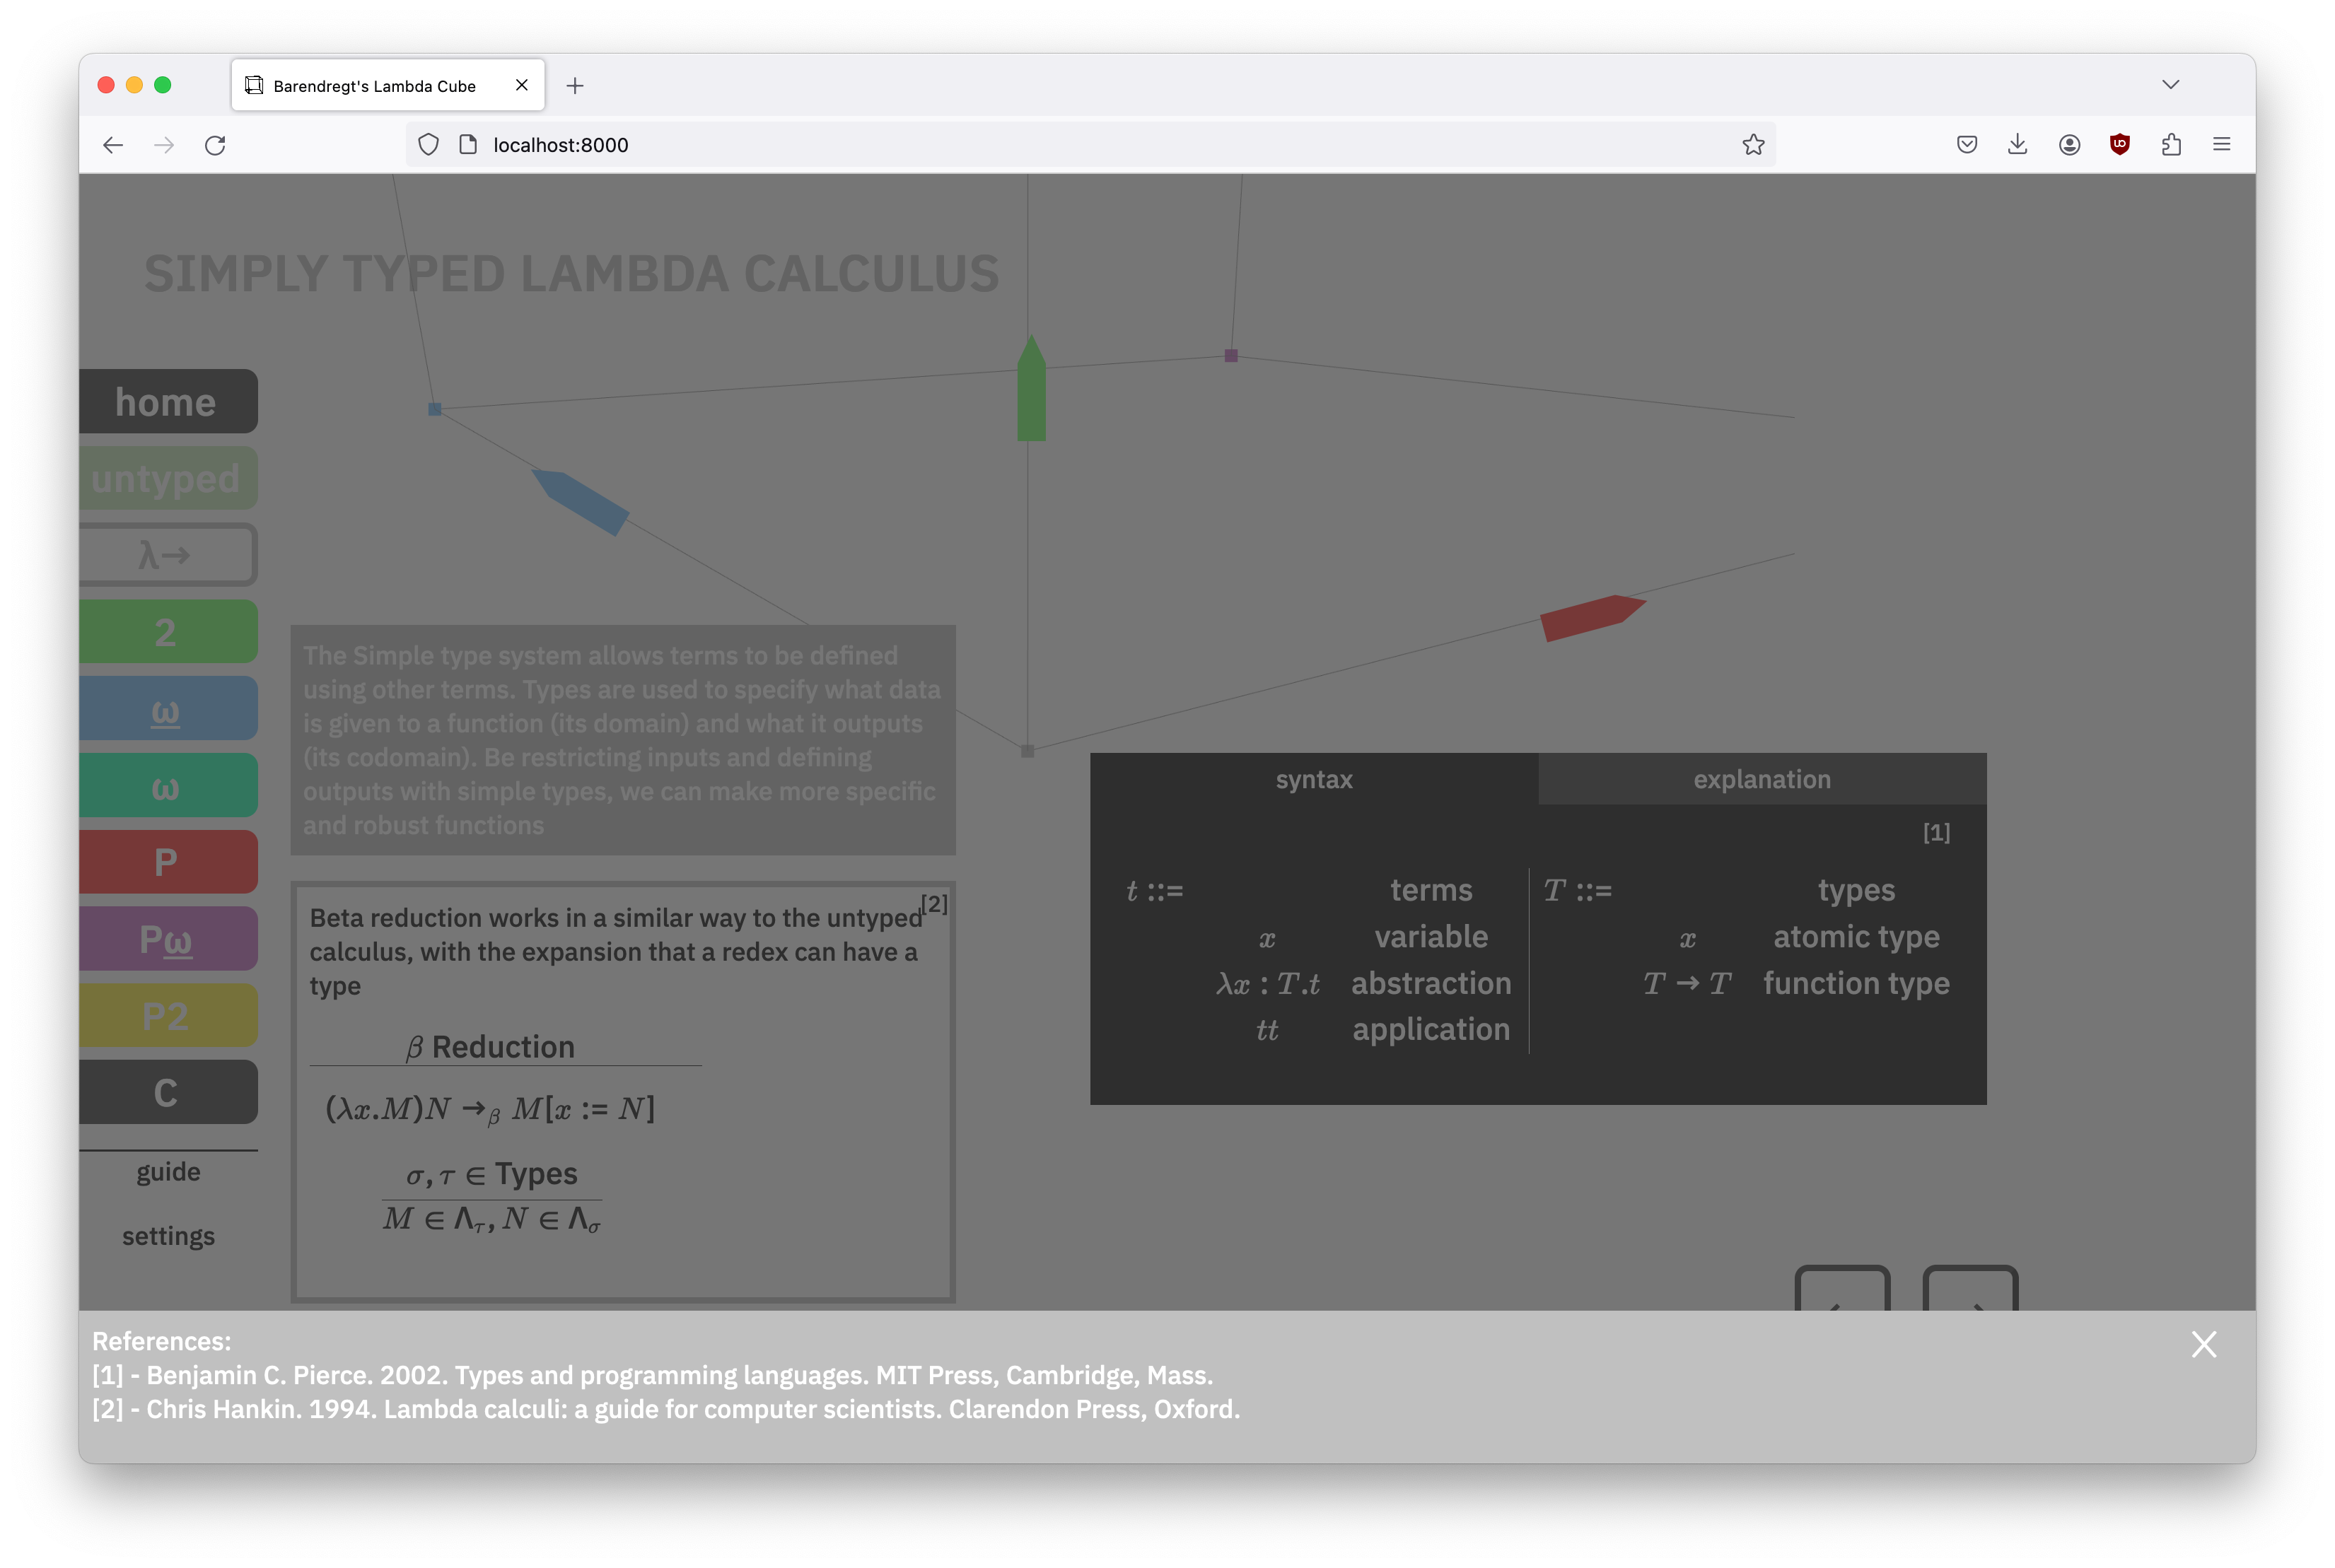
\includegraphics[width=0.8\linewidth]{dissertation/images/final_citations.png}
    \caption{An example of the HTML generated by the view function}
    \label{fig:enter-label}
\end{figure}

There are also files such as System or Color.elm, which do not directly compile into HTML, but instead help by defining parameters, types and helper functions which are used by other files.  Examples from System.elm are shown beneath.

\begin{lstlisting}
    type System
    = Home
    ...
    | Two

color : System -> Color
color sys =
    case sys of
        ...
        Two ->
            green

toString : System -> Html msg
toString sys =
    case sys of
        ...
        Two ->
            b [] [ text "2" ]

toggleProperty : Property -> System -> System
toggleProperty property system =
    case ( system, property ) of
        ...
        ( Two, Polymorphism ) ->
            Simple


hasProperty : Property -> System -> Bool
hasProperty property system =
    case ( system, property ) of
        ...
        ( Two, DependentTypes ) ->
            False
\end{lstlisting}

The definitions of these functions are kept in one file instead of being defined ad hoc throughout the program.  This is so I can more effectively keep track of functions which derive state from the system.

One persisting problem during the implementation phase was finding enough space on the screen to display all of the information, while occluding as little of the cube as possible.  This was most obvious in displaying the typing rules of each node, which took up a large amount of space.  My first solution to this was to find a space where the div fit, and making it scrollable.  This was a helpful solution, however I still required more space to be able to show all the information which I thought to be necessary.  I then implemented a tab system to the syntax box, where the user could click between the EBNF syntax and an explanation of the typing rules. The result of which is shown beneath.

\begin{figure}[h!]
    \centering
    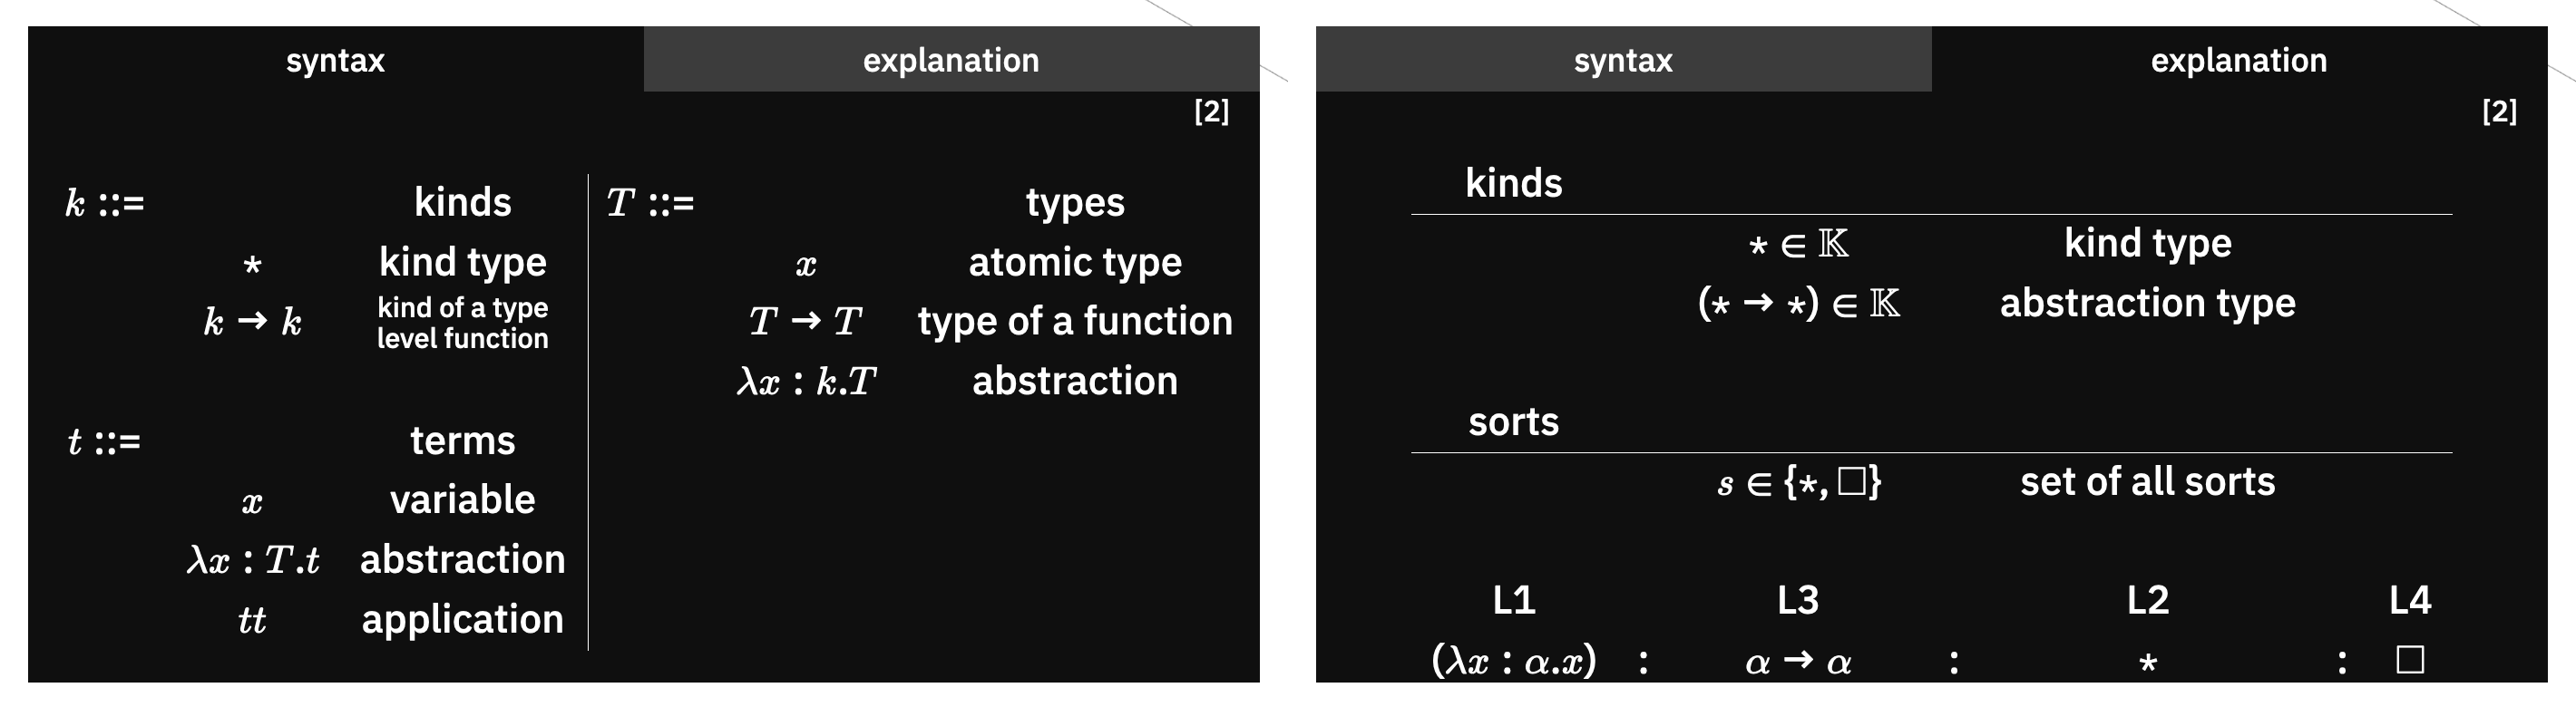
\includegraphics[width=0.8\linewidth]{dissertation/images/syntax_collage.png}
    \caption{An example of the two different views of the syntax box}
    \label{fig:enter-label}
\end{figure}

I achieved this by adding a new boolean to the model, where true and false determined which of the compiled .tex files would be displayed, and a new message \texttt{SetSyntax} which toggles the state of the boolean.  An approach which aligns more to functional programming paradigms would have been to define a custom type that determines which version to show, such as:

\begin{lstlisting}
    type SyntaxContent
    = Syntax | Explaination
\end{lstlisting}

This is a better approach as it stops the problem of boolean blindness, which is when too many parameters are boolean values when `richer' code structures are available.  This can cause confusion for the programmer as they struggle to make sense of multiple similar seeming inputs, and is generally a less information dense method than is otherwise achievable.  It is also more readily scalable, as a third or fourth type variant could be added easily, and the box made to select the file to display based on that.

In order to help build recognition of the names of the types and systems, I decided that the buttons that allowing users to click on the nodes, and arrows used to transfer the user between nodes should have their name pop up when the user moves their mouse over them.  The first way that I implemented this on the cube's corners was to use the \texttt{onMouseEnter} and \texttt{onMouseLeave} attributes of Elm's Html.Events package.  This implementation used a message that was sent every time the mouse moved over the specific element, which updated a new instance of the type System model, called 'over'.  This value was used to determine if the name of the node was showing or not, with a simple 
\begin{lstlisting}
if system == over then system.toString sys else div [][]
\end{lstlisting}

This was a workable solution, however it introduced a very transient value to the state, and would not work for the arrows, as they did not have a specific type which could be updated with a message in the same way.

The solution to both of these problems was to use CSS classes.  By using CSS's hover selector, and redefining the div that contains the arrows to have class arrow-container, I was able to change what text is shown on screen without having to use the model message update system.  The code for the arrows is shown beneath.

\begin{lstlisting}
    .arrow-container:hover>.arrow-text {
      display: block;
    }

    .arrow-container>.arrow-text {
      display: none;
    }
\end{lstlisting}

\section{Using WebGL}

Using WebGL was initially quite difficult, due to the relatively low level of detail in the package's documentation.  There were very few details that I was able to find about the specifics of the camera and the uniforms, which made it difficult to get the project into a compilable state.  However, there were some useful examples listed on the repository which I ended up using to learn how to use the package.

Each mesh is passed a 'uniform' which determines its rotation, angle, perspective and details about the camera and colour it is shown in.  I used this to give the constant animation to the cube, by constantly rotating it on each axis by the sine of the elapsed time since the page was opened.  A sine function was essential here to limit the maximum movement of the cube, and to make sure that it moves on a closed track.

At this stage, I had a version of the cube that was fully rendered and navigable.  However, when moving from node to node, using either the sidebar or the transfer arrows, the camera would instantly teleport to the new position.  While this is an acceptable solution and computationally efficient, it gives a sense of disconnection to the cube, as you never move around the cube organically, just jump from point to point.

The solution to this was to linearly interpolate camera positions between where the camera was before the system was updated, and the position that it should end up in the new position.  Doing this would necessitate storing the eye and target variables of the camera in the system, as they would need to be constantly re-evaluated while the camera was en route to its new position.

\begin{lstlisting}
vec3lerp : Vec3 -> Vec3 -> Vec3
vec3lerp from to =
    let
        newX =
            lerp (getX from) (getX to)
        newY =
            lerp (getY from) (getY to)
        newZ =
            lerp (getZ from) (getZ to)
    in
    vec3 newX newY newZ

lerp : Float -> Float -> Float
lerp from to =
    from + 0.15 * (to - from)
\end{lstlisting}

The function `vec3lerp' takes the two positions 'from' and 'to'.  The camera movement could need to be linearly interpolated in all three dimensions at once, so all three of the dimensions are linearly interpolated using the 'lerp' helper function.

The function 'lerp' takes two floats, and adds 0.15 times the difference between the second and the first float to the first float.  The value of 0.15 changes how quickly the camera moves to the new position, and was chosen to be slow enough to be noticeable, but not so slow that it was annoying and wasted the user's time.

The 'Tick' message was then updated to change the camera and eye component to a version of themselves with 'vec3lerp' applied to them selves.  This means that the camera is technically always moving, but it is imperceptible after a certain point, especially in conjunction with the cube's movement.  For this reason, the code to move the camera is in the Home.elm file, where the messages are defined, rather than with the rest of the code about the cube and animation stored in Cube.elm.

\section{LaTeX2Elm Translator}

The implementation of my translator, stored in the latex2elm.js file, remained mostly unchanged during the implementation phase of my project.  The program is quite minimal, defining just two functions to convert the code first from .tex format to HTML, and then into Elm.  The main process of the file is shown beneath.

\begin{lstlisting}
Promise.all(Deno.args.map(async infile => {
    let moduleName = path.parse(infile).name[0].toUpperCase() +                     path.parse(infile).name.substring(1)
    const latex = await Deno.readTextFile(infile)
    const elm = latex2elm(moduleName, latex)
    await Deno.writeTextFile("gen/MathML/" + moduleName + ".elm", elm)
    console.log("generated", moduleName + ".elm")
}))
\end{lstlisting}

The first step in the process is to read the file name, and to make sure that it is in the correct format for an Elm module it is given a leading capital letter.  Then the content of the .tex file is read using Deno's \texttt{readTextFile} function.  Then, the function latex2elm is called.

\begin{lstlisting}
function latex2elm(moduleName, latex) {
    let html;
    try {
        html = katex.renderToString(latex, { output: "html" })
    } catch (error) {
        console.error("[Error] " + error.rawMessage)
        return `text "error: ${error.rawMessage}"`
    }
    const parser = new DOMParser()
    const dom = parser.parseFromString(html, "text/html")
    const output = `
module MathML.${moduleName} exposing (view)

import Html.WithContext exposing (text, node)
import Html.WithContext.Attributes exposing (attribute)
import Context


-- this code was generated by latex2elm

view = ${domToElm(dom.body.children[0])}
`
    return output
}
\end{lstlisting}

This function uses an imported KaTeX library to convert the .tex file into a list containing both MathML and HTML compiled DOMs.  I then define a string which has the header template of an Elm file (lines 11 → 19), where I set the file up to be properly exported, import the necessary packages, and add a comment to say that this file has been automatically generated.

The Elm file's view function is then defined, by passing the first element (the compiled MathML DOM) to the function function \texttt{domToElm}.  This string is then returned, and written to the new file.

\begin{lstlisting}
function domToElm(node) {
    if (node.nodeType == 3) {
        // text node
        return `text "${node.textContent.replaceAll('\\', '\\\\').replaceAll("\n", "")}"`
    }

    if (node.nodeType == 1) {
        // normal node
        const children = [...node.childNodes].map(domToElm)

        const attribues = []

        for (let attr of node.getAttributeNames()) {
            attribues.push(`attribute "${attr}" "${node.getAttribute(attr)}"`)
        }

        return `node "${node.localName}" [ ${attribues.join(", ")} ] [ ${children.join(", ")} ]`
    }
}
\end{lstlisting}

\texttt{domToElm} is defined recursively, where as long as the node is not the end of file, the \texttt{domToElm} maps itself over the node's children, and returns the result.

The steps where the file is actually opened, compiled and save are wrapped in a Promise block. This is done so that instead of manually passing files in one at a time, an editor can simply call the file on an entire folder at a time, and every .tex file will be read and compiled sequentially.  The files themselves are read in asynchronously, and the steps described above are mapped over them.

\section{Deployment}

An initial requirement of my project was to be usable by the School of Computing to help teach some concepts in Theory of Computation.  For this purpose, the website would need to be hosted on the University's network.  To make sure my website was suitable for this purpose, I made a trial deployment to GitHub Pages.  In doing so, I discovered some faults with my website that had not occurred to me while using only my computer to program it.

The first fault that I noticed was that the web page was not portable between all browsers.  I had been using Mozilla Firefox to test my website up until this point, but once I used it on a lab computer running Google Chrome, there were problems immediately visible.  Firstly, my custom fonts failed to load, but more critically so did the EBNF syntax.  This was a major issue since it contains some of the most important information on the website.

In order to fix the fonts issue, I had to add to add the font into my index.html file as a default.  Chrome and Safari do not properly accept inheriting fonts in Elm like Firefox does, which was not mentioned in any documentation I was able to find.

\begin{lstlisting} [caption={Importing and setting the font "IBM Plex Sans" globally}]
    * {
      font-family: "IBM Plex Sans", sans-serif;
    }
    
    @font-face {
      font-family: "IBM Plex Sans";
      src:
        url("fonts/IBMPlexSans-Medium.woff2") format("woff2");
      font-weight: normal;
      font-style: normal;
    }
\end{lstlisting}

Upon inspecting a div which should contain the rendered maths, I discovered that all the content was there, but had failed to render.  Through trial and error I found that if wrapped in a math block, like the files generated by my translator, only Firefox was able to render the MathML code.  However once outside of that block, the equations were able to render correctly in all browsers.  I fixed this by editing the header text in my compiler to remove the Math block.  Again, this was not explained in any documentation I could find.

When I was creating the site, I hard coded the dimensions and location of every element on the screen in terms of pixels.  While the website looked fine on my computer, the whole site was much too small or large on screens with different resolutions to mine, and it could not account for the screen being resized.  To fix this, I implemented a function to convert the pixel measurements I had designated to a string which would be interpreted in the style tag as a number of view widths.  The code to do this is as follows.

\begin{lstlisting} [caption={The implementaion of the px function in Utils.elm}]
px : Int -> String
px n =
    String.fromFloat (toFloat n / 17) ++ "vw"
\end{lstlisting}

I then universally applied this function wherever a pixel measurement was given using a regular expression in find and replace.

\section{Summary}

\begin{figure}[h!]
    \centering
    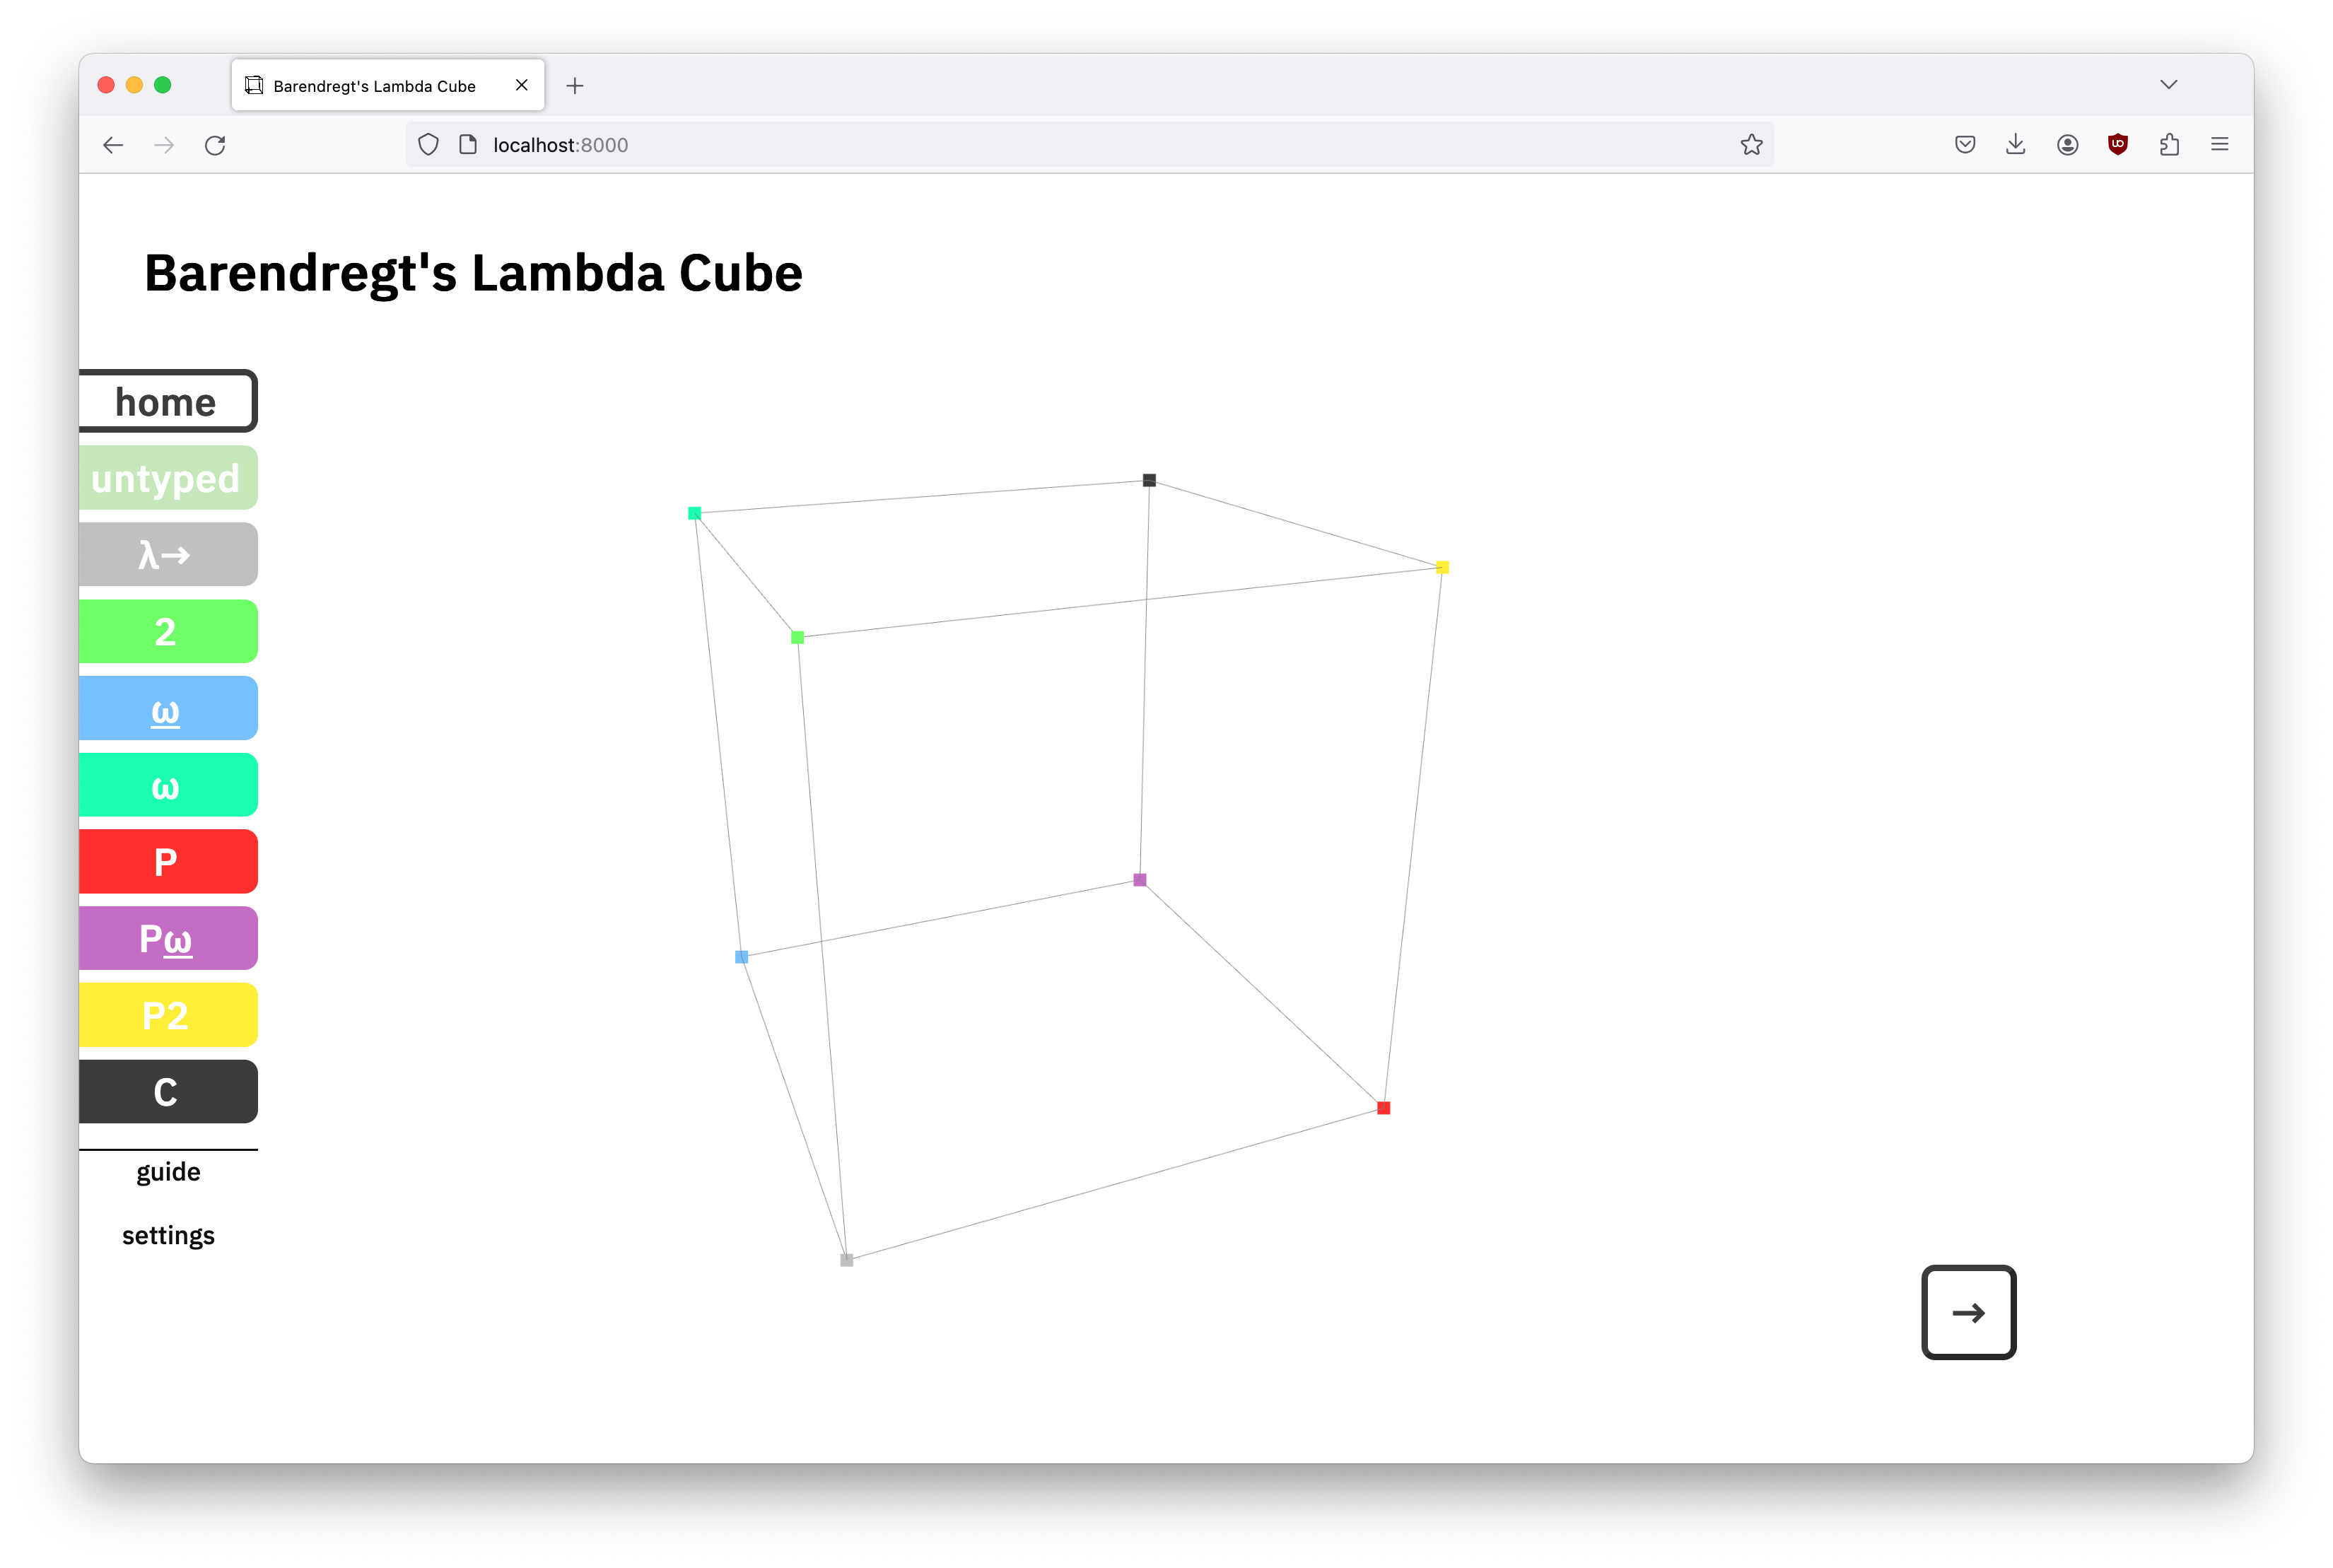
\includegraphics[width=0.8\linewidth]{dissertation/images/final_home.png}
    \caption{The home view of the final state of the website.}
    \label{fig:enter-label}
\end{figure}

\begin{figure}[h!]
    \centering
    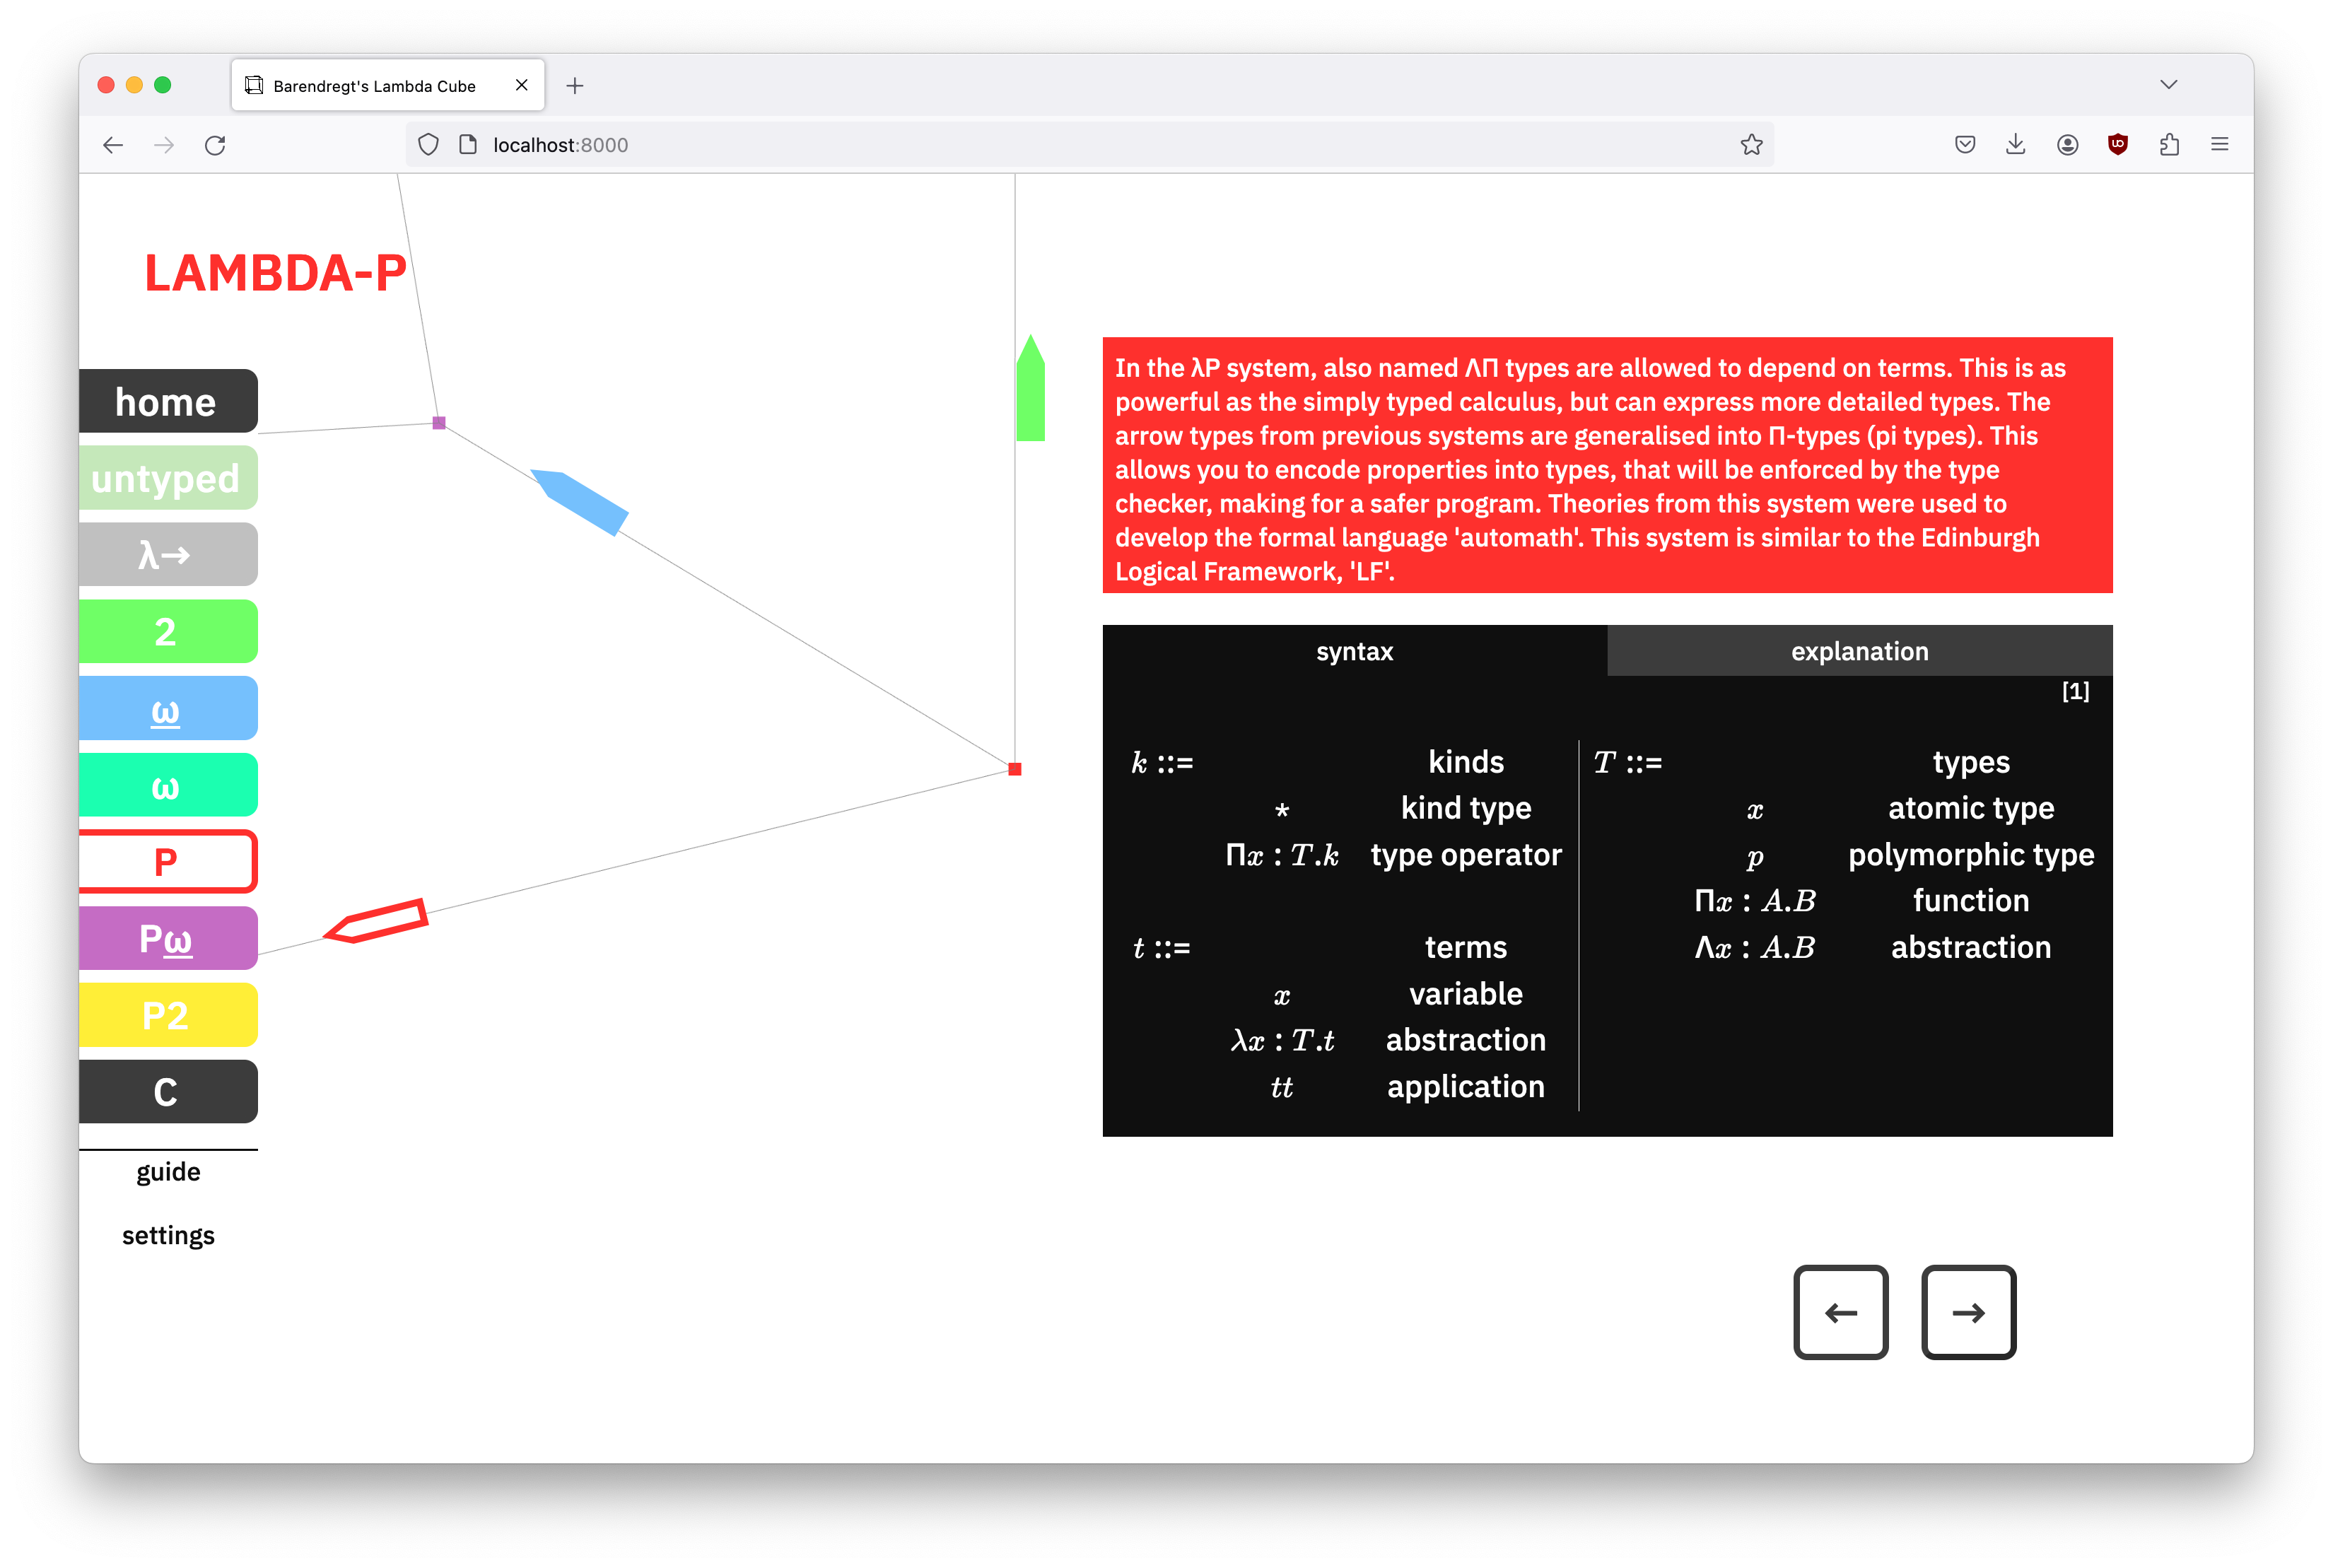
\includegraphics[width=0.8\linewidth]{dissertation/images/final_zoomed.png}
    \caption{An example node of the final site being viewed}
    \label{fig:enter-label}
\end{figure}

Many of the difficulties which I had with the implementation of my design were due to inadequate documentation.  This meant that I had to spend a large amount of my time using trial and error, changing parts of my code attempting to solve the problem.  If the specifics of systems like WebGL's camera, or quirks such as the font's not being inherited in browsers other than Firefox were explained, I would have been able to spend less time solving each issue.

I would have liked to keep the model as minimal as I had planned in the design phase, however the increases in scope necessitated increasing the complexity of the model.  I believe that the features I was able to deliver make up for the more complex model, and that I have written my code in a way which is straightforward enough that the complexity of the model and messages is not an issue.

It was very helpful to make a test deployment of my site, as it allowed me to easily test the page on other browsers and screen resolutions.  During this process I was able discover faults in my code, such as the font non inheritance, as well as places where I could improve quality and efficiency, such as removing the Math block or switching to view widths instead of using pixels.

I did have to bypass Elm's architecture using CSS and JavaScript three times, however I believe that each time was justifiable, as the alternative ways using only Elm that I tried added a greater amount of complexity.
%==================================================================================================================================
\chapter{Evaluation} 

\section{University Accessibility Guidelines}

As the website was partially designed to be used by the University of Glasgow, It should be able to be used in a course which adheres to the University's "Accessible and inclusive learning policy" in order to be for that requirement to be met. According to the University's website, the three most common accessibility issues with content are: PDFs being made from poor quality scans or inaccessible documents, no alternative text for images and poor colour contrast making text difficult to read \citep{accessible_inclusive}.

As my website did not display or generate either PDFs or images, it is not subject to the first two issues.  However, as colour is used as a major design element, it is potentially vulnerable to the third.  Using Google Chrome's 'Lighthouse' software, I was able to test how accessible the colours of my website were.  Lighthouse found two instances where the colours used were seen as incompatible: The simply typed lambda calculus where content was delivered in white text against a grey background, and system P2, where white text is used against a bright yellow background.

In response to this, I changed both the grey and yellow colours to be darker, increasing the contrast and making the text easier to read.  As well as this, I made the text on the yellow background bold, which again aids in visibility.  I decided not to switch away from using yellow, as I believe that it has a larger benefit in making the screen more interesting to look at than the damage it does in readability, especially considering the relatively sparse content at the P2 system due to the lower level of research which has been undertaken into that node.

The University also has a page on its "Digital Accessibility guidelines" \citep{digital_accessibility}, which describe a set of guidelines "adapted from the SCULPT for accessibility guide developed by Helen Wilson, Digital Designer at Worcestershire County Council." \citep{sculpt}.

Most of these are not relevant to my project, as they discuss the use of hyperlinks, tables and hosted images, however much of the information regarding plain text is useful.  The main points are to: 

\begin{itemize}
    \item 
\end{itemize}
Make sure the text is left-aligned, Use double or 1.5-line spacing, Use sentence case, Avoid underlining, Do not use colour alone to get across meaning, Avoid footnotes where possible and to use at least 12 point size of a sans serif font.

My website complies with most of these points, however does not use 1.5 line spacing or 12 point font universally, as all of the content on the website scales with the screen width, including font size.  1.5 line spacing is also not used, as I need to make most efficient use of the limited space afforded to me.

\section{Assessing My Requirements Process}

User stories were useful for deriving the initial requirements, but I soon progressed past them, and never decided to reassess any.  Instead, I assessed the project itself to see what I was missing from it.  Later, once it was far enough along its development cycle, I ran user trials as detailed later in this chapter.  These observed how the website was used, and how effective it was at teaching the users.  If I was to start a similar project, I do not think that I would use user stories.

I did not find MoSCoW prioritisation to be very useful.  This was because many of the features that needed to be implemented rely heavily on each other.  For instance, you cannot add citations before you have the text that is being cited.  This means that instead of following the order of tasks set out at the beginning of the project, I worked on most of the areas of the project simultaneously, prioritising tasks based on what I was most interested in at that moment in time.  I also found granularity to be an issue, as the requirements were to broad to make the best use of the prioritisation structure, and as all of the requirements were either must-have or should-have, there was not enough distinction between the two categories.

Towards the end of the project, I created a GitHub issue for each task I still had remaining, and closed these issues only when I committed the code for the solution.  This was a much more effective way of managing my priorities, as I always had a clear idea of how much left to do, and exactly what tasks I should be working on.

If I were starting the project again, I would use GitHub issues from the start and try to define more granular and independent tasks, as well as prioritising them using story points or an explicit calendar of when I would want each task to be completed.  I believe that a more concrete timeline would have helped me to complete tasks in a shorter time frame, and in a more productive order.

By having a more complete product earlier in the development cycle, I would have been able to discover more of the issues related to deployment sooner and could have made a better website as a result.  It would also have been possible to conduct multiple rounds of user studies, which would have let me verify whether the changes I made were beneficial or not.

\section{Experiment Methodology}

In order to assess how effective my website was at teaching people concepts from the lambda cube, I ran a set of user studies on students who were already familiar with some basic concepts of programming languages.  I chose this subset as they are the primary intended audience for the website once it is launched.  If I had used an audience unfamiliar with the concept of lambda calculus then they could spend too long learning the basics at the untyped lambda calculus node to effectively have time to explore the cube itself.

I managed to find ten students who had previously taken the Programming languages course who were willing to take part in my study.

The study I planned to run was split into two parts.  Firstly the user would be given 15 minutes to use the website, while I observed and made notes on how they used it.  Then the user would be given a questionnaire to fill out without using the website.  The questionnaire had four sections:

\begin{itemize}
    \item First, the user would be asked to rank themself based on their confidence in three different areas of prior knowledge: Knowledge about lambda calculus, Familiarity with BNF syntax and familiarity with formal logic.  By collecting this data, I would have enough background about each student to be able to draw conclusions from their results in the next parts of the survey.

    \item Next, they would be given a wireframe of the lambda cube and of its axes, and be asked to label the corners of the cube and the type systems represented by the axes.  This is the most basic information about the lambda cube, so by giving them a simple recall task I would be able to tell how effective the website is at teaching the fundamental concepts of the cube.

    \item After this, the respondent is given three more complex recall questions, asking about specific features of some of the systems, and giving them a few lines to write an answer to each.  By having some longer questions about deeper topics, I could see how effectively my website is able to express more complex aspects of the lambda cube.

    \item Finally, there is a section where the user is directly asked for feedback, both by ranking the site in terms of legibility, information quality, information depth, feature richness and aesthetics, and a section where they were free to write any feedback or suggestions they had.  By having both of these two sections, I could gather quantitative and qualitative feedback, diversifying the types of feedback I could use.
\end{itemize}

To determine how long to let the user study the website before testing them, I timed myself reading all of the content on the website at a normal pace, and then doubled this value in order to account for my familiarity with the content.

I used my trial deployment of the website to run the tests on, as it meant that I could keep this version of the site the same throughout all of the tests, and be implementing feedback gathered from the tests in real time.  This ensured that the results would be internally consistent, and that I would not forget minor corrections or suggestions that I wanted to make because I was able to make the alterations straight after each trial.  Screenshots from the deployment which the tests were run on are shown beneath.

\begin{figure}[h!]
    \centering
    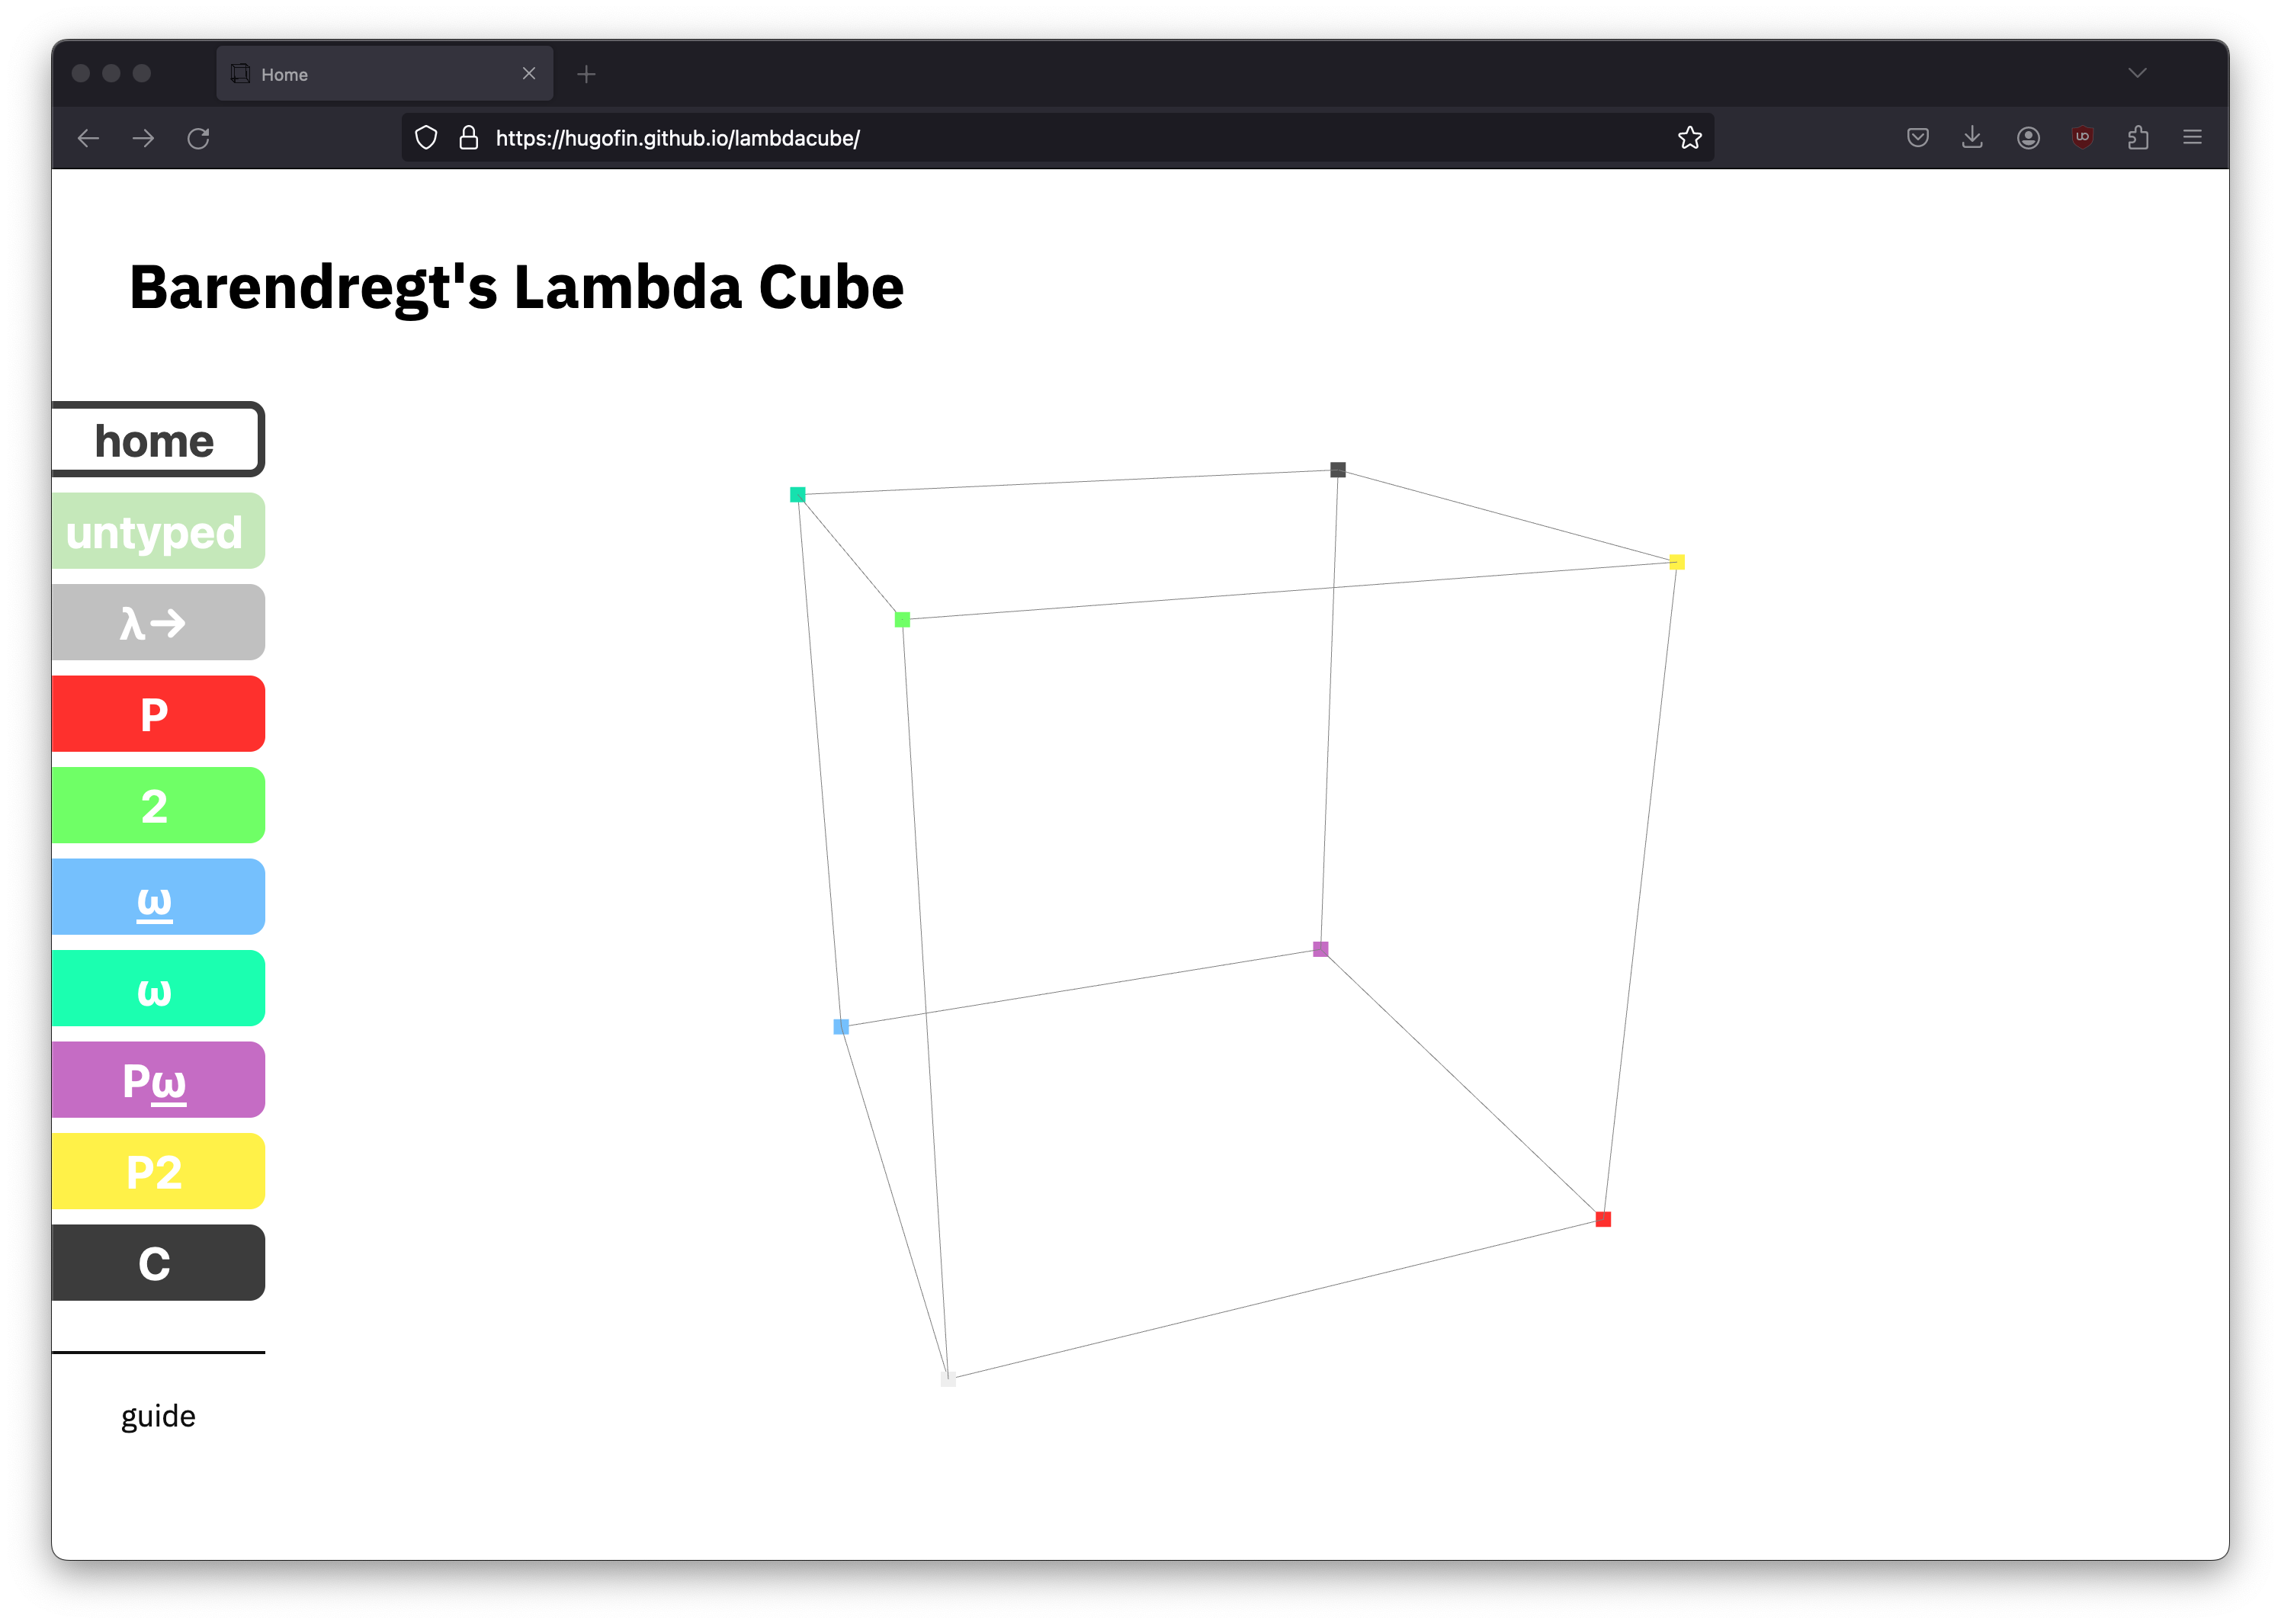
\includegraphics[width=0.8\linewidth]{dissertation/images/trial_deployment_home.png}
    \caption{The home view of the deployed site.}
    \label{fig:enter-label}
\end{figure}

\begin{figure}[h!]
    \centering
    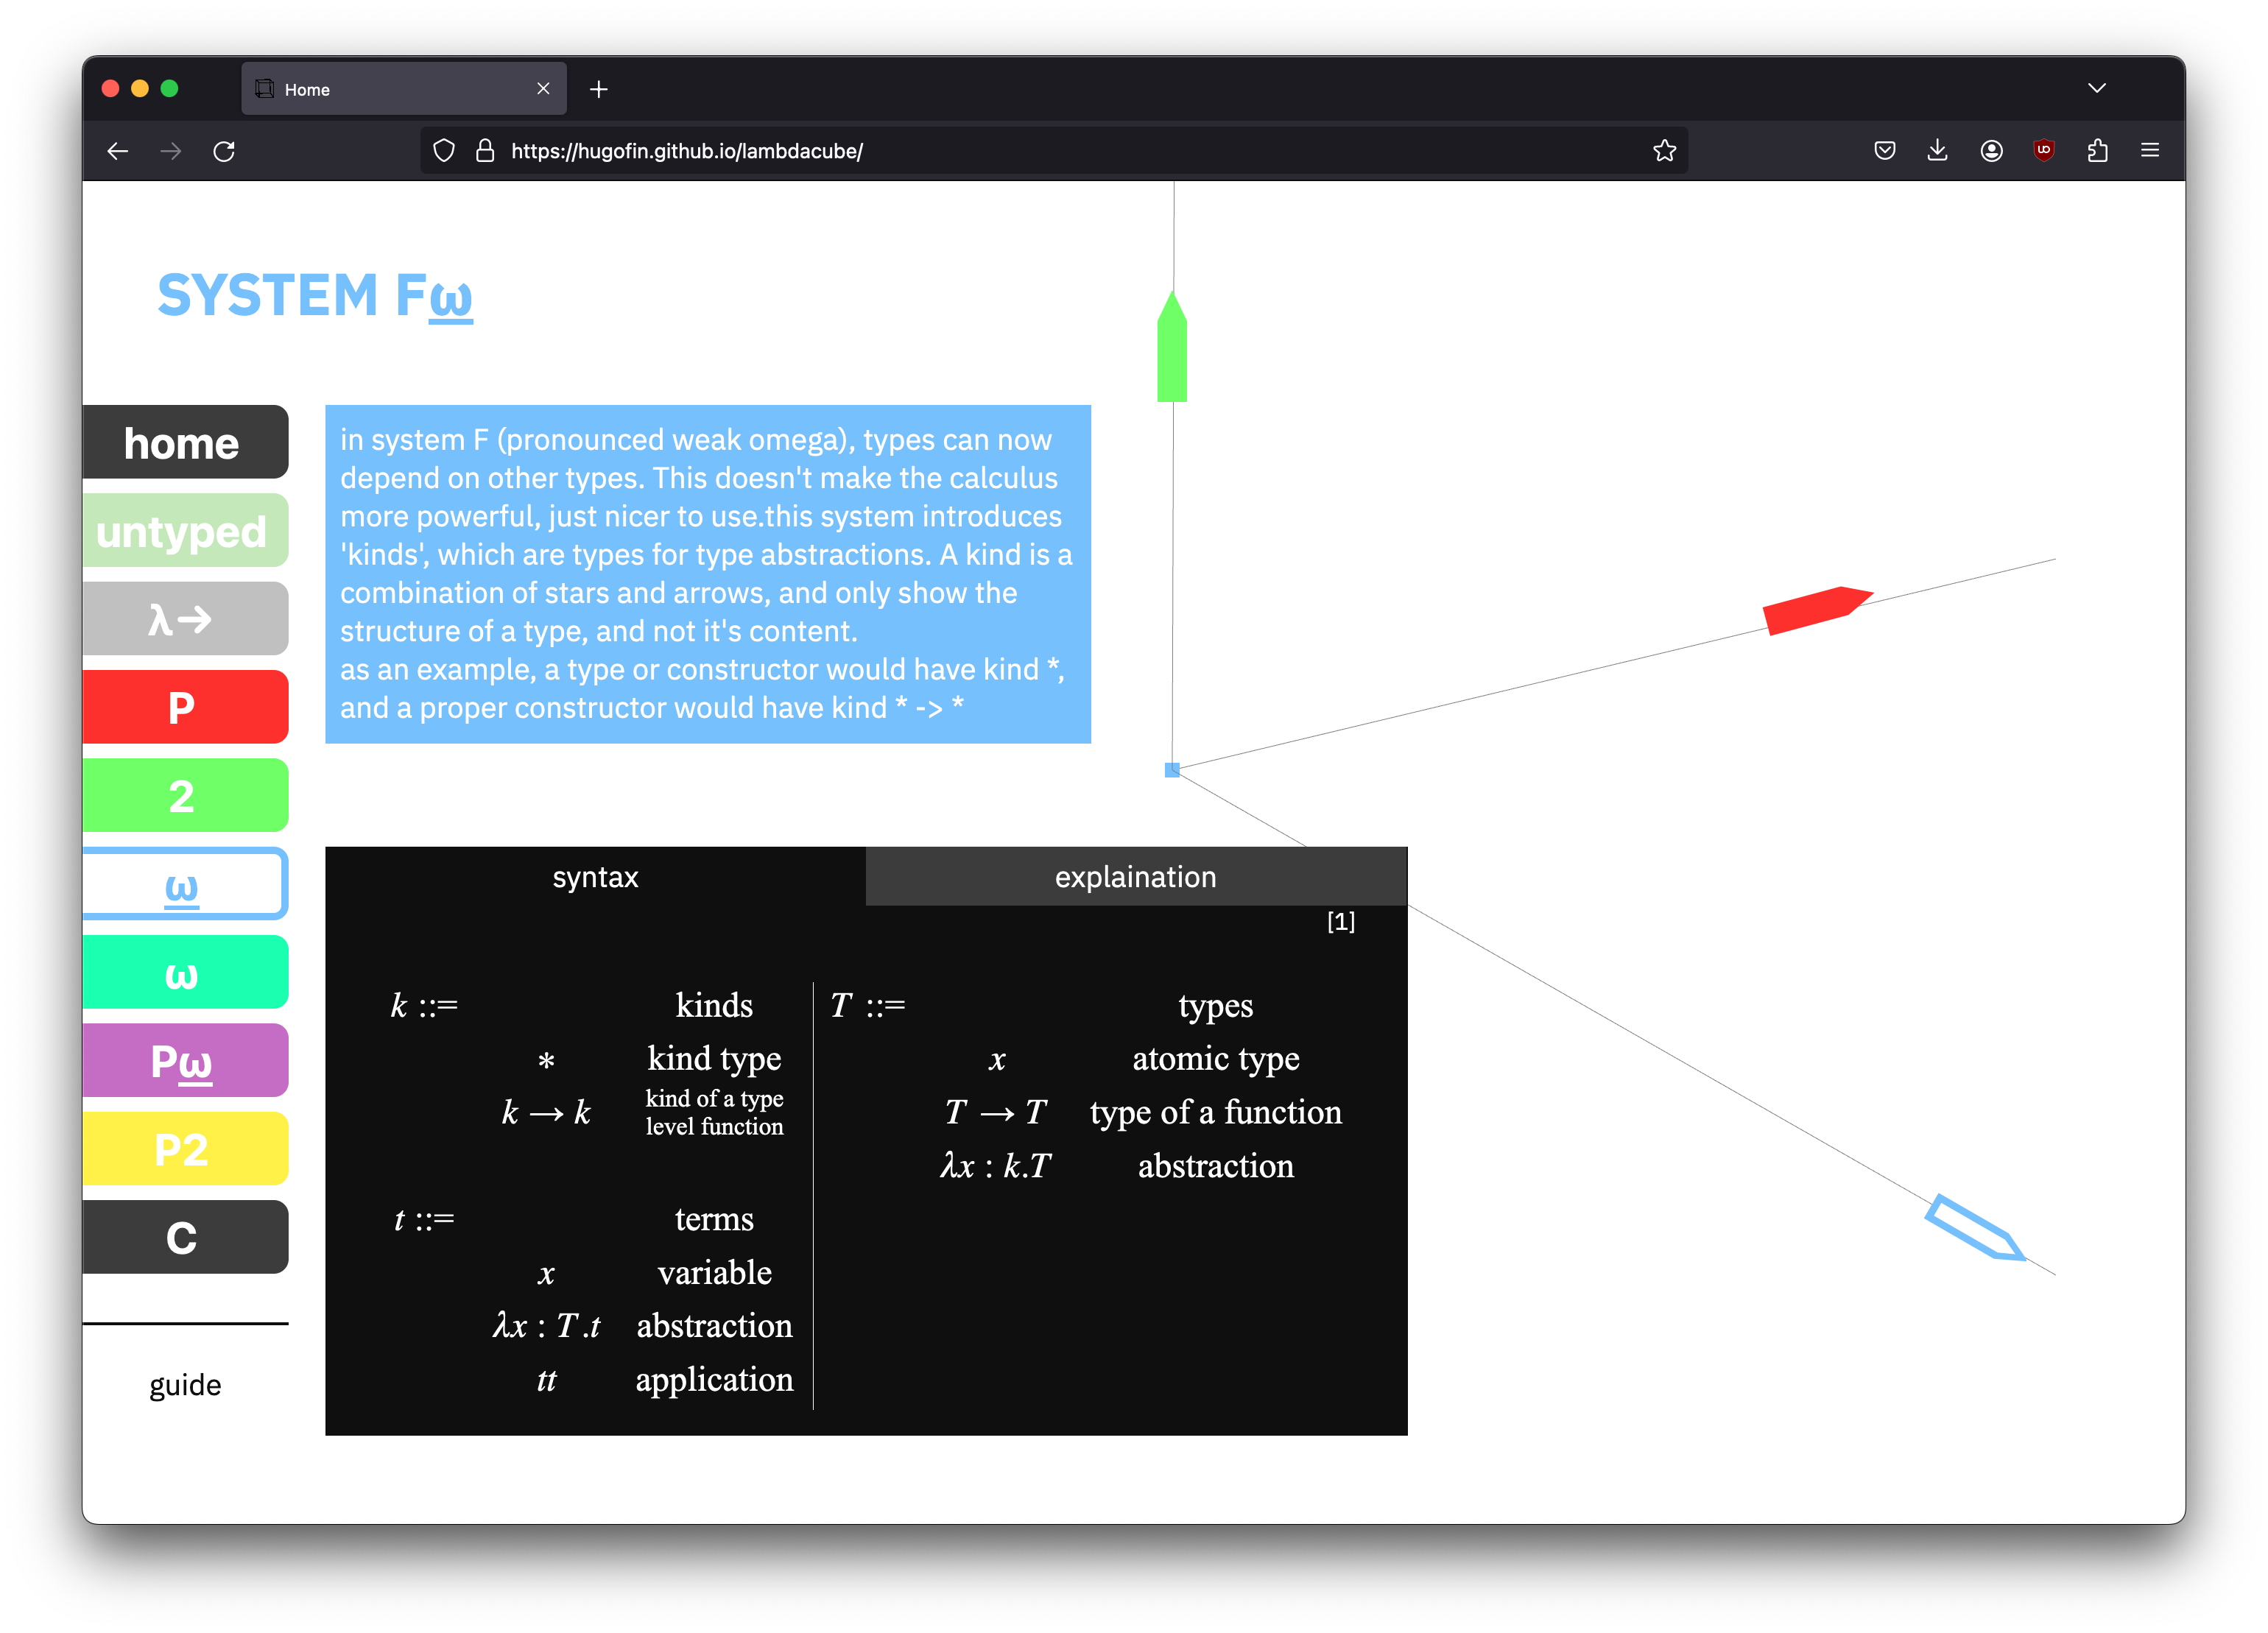
\includegraphics[width=0.8\linewidth]{dissertation/images/trial_deployment_zoomed.png}
    \caption{An example node of the deployed test site being viewed}
    \label{fig:enter-label}
\end{figure}

\section{Study Results}

\begin{table}[!ht]
    \centering
    \begin{tabular}{|p{3cm}|l|l|l|l|l|l|l|l|l|l|l|}
        \hline
        ~ &  № 1 &  № 2 &  № 3 &  № 4 &  № 5 &  № 6 &  № 7 &  № 8 &  № 9 &  № 10 & Average \\ \hline
        Confidence Scores & ~ & ~ & ~ & ~ & ~ & ~ & ~ & ~ & ~ & ~ & ~ \\ \hline
        Understanding of Lambda Calculus & 2 & 4 & 0 & 2 & 1 & 0 & 0 & 0 & 1 & 3 & 1.3 \\ \hline
        Ability to read BNF Syntax & 0 & 4 & 1 & 3 & 1 & 1 & 2 & 3 & 2 & 4 & 2.1 \\ \hline
        Formal Logic & 8 & 6 & 4 & 6 & 2 & 3 & 3 & 6 & 4 & 5 & 4.7 \\ \hline
        Quiz Scores & ~ & ~ & ~ & ~ & ~ & ~ & ~ & ~ & ~ & ~ & ~ \\ \hline
        Cube corner task & 2 & 4 & 2 & 6 & 6 & 2 & 6 & 1 & 2 & 5 & 3.6 \\ \hline
        Axes task & 1 & 1 & 0 & 3 & 2 & 2 & 1 & 1 & 2 & 3 & 1.6 \\ \hline
        Kinds & 0.5 & 0 & 1 & 1 & 0 & 0.5 & 0 & 2 & 0 & 2 & 0.7 \\ \hline
        Pi types & 0 & 1 & 0 & 1 & 1 & 1 & 1 & 1 & 0 & 1 & 0.7 \\ \hline
        Unexplored systems & 0 & 2 & 1 & 2 & 1 & 0 & 1 & 0 & 1 & 0 & 0.8 \\ \hline
        Rating & ~ & ~ & ~ & ~ & ~ & ~ & ~ & ~ & ~ & ~ & ~ \\ \hline
        Legibility & 9 & 7 & 10 & 6 & 8 & 8 & 9 & 7 & 8 & 7 & 7.9 \\ \hline
        Quality of information & 10 & 8 & 7 & 9 & 7 & 8 & 8 & 8 & 9 & 7 & 8.1 \\ \hline
        Depth of information & 10 & 8 & 8 & 8 & 7 & 5 & 10 & 5 & 7 & 8 & 7.6 \\ \hline
        Number of features & 7 & 5 & 10 & 7 & 10 & 10 & 5 & 6 & 7 & 6 & 7.3 \\ \hline
        Look and feel & 8 & 8 & 9 & 7 & 7 & 8 & 8 & 10 & 9 & 8 & 8.2 \\ \hline
    \end{tabular}
    \caption{A table containing the full results of each of the user studies}
    \label{fig:enter-label}
\end{table}

Above is the table of results for each of the user studies.  One common theme through all of the studies was the relatively low score in the questionnaire, with the highest score being 41 percent of the possible maximum.  This is most likely a result of the relatively short time allotted to the user to explore the website when compared to the difficulty of the subject matter.  This is evidence is backed up by the graph seen beneath, where the user's self reported prior knowledge is plotted against their score in the quiz section.

\begin{figure}[h!]
    \centering
    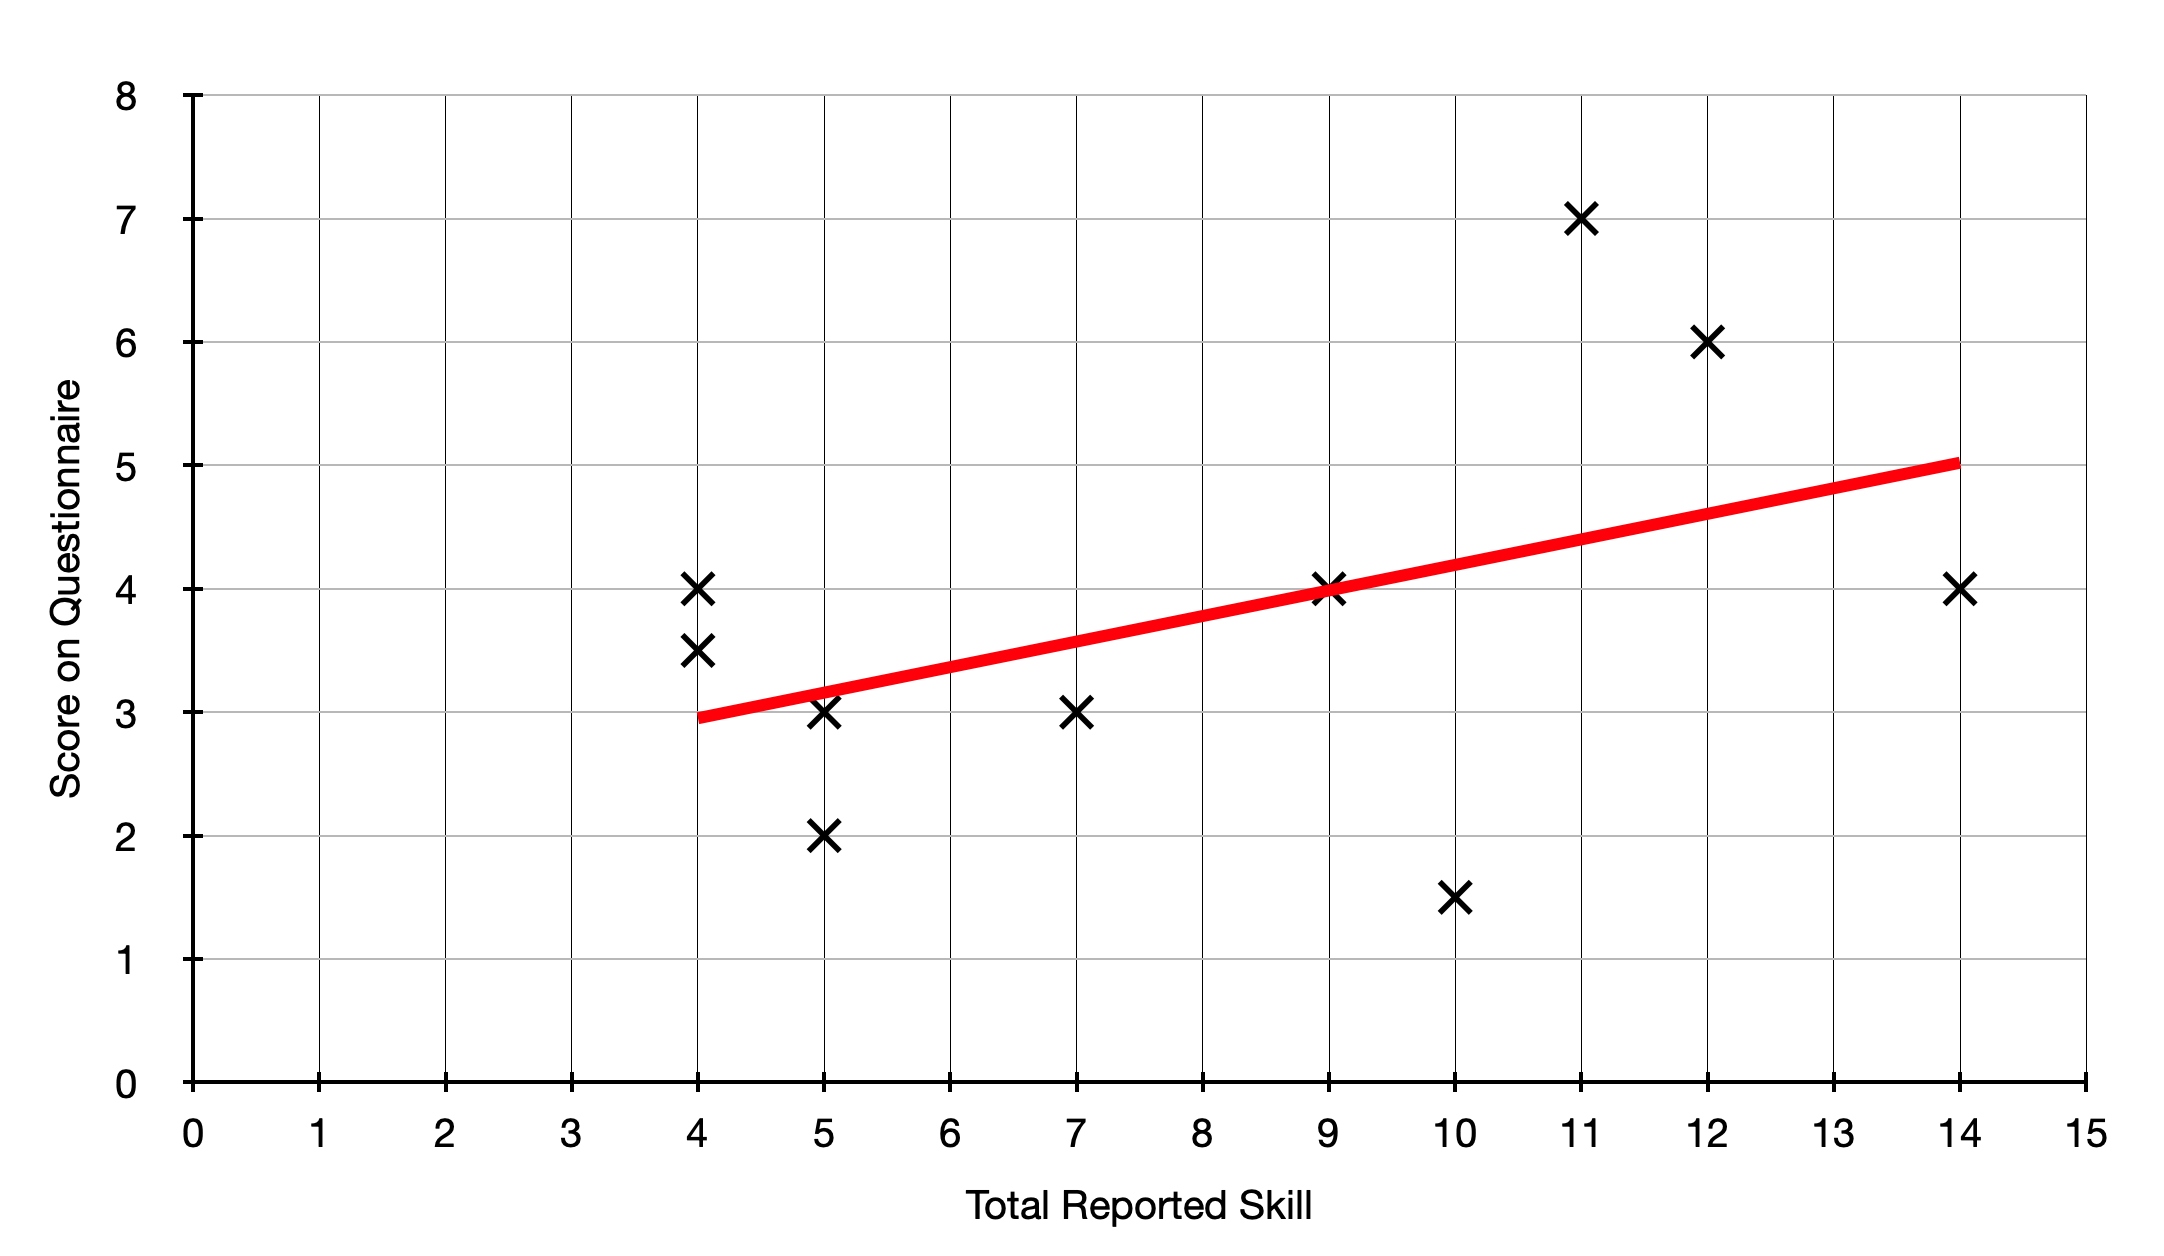
\includegraphics[width=1\linewidth]{dissertation/images/skill_against_score.png}
    \caption{A graph showing each users confidence plotted against their score in the questionnaire, with the line of best fit demonstrating a positive correlation between the two measures}
    \label{fig:enter-label}
\end{figure}    

This graph shows a positive correlation between knowledge in the background areas which I identified, and score in the test.  This, combined with the very low confidence reported by most of the users studied would suggest that the scores on the assessed portion would be generally low.

Another possible explanation could be that the Programming Languages course previously studied by the participants did not have sufficient background to prepare the users for this study, as notable elements such as beta reduction and typing rules were absent from the curriculum. 

However it could also be that my website was not very good at teaching the concepts I had hoped to explain.  This should definitely be considered as a reason, however I believe that it is less likely than the reason discussed above, because no part of the questionnaire was failed by every user.  From this, we could conclude that the website is effective enough to teach the content which it contains, and instead the study was flawed.

The section of the questionnaire where I asked directly for feedback was perhaps the least informative.  There were generally very high results, with no user ranking the site worse than a five out of ten in any of the aspects I asked about.  The quality of the website which received the lowest overall ranking was "number of features", as some users noted that there were not settings which they would expect the website to have.  Depth of information was also criticised, mostly in so far as the guide was not detailed enough to be able to answer all of their questions.

\section{Changes I made}

The first thing I noticed was that the vast majority of users who I surveyed chose to approach the website by clicking each system in the sidebar in order, not navigating using the arrows or clicking on nodes to go to them.  This was not necessarily a problem, however the order of the buttons in the sidebar was chosen somewhat arbitrarily, and was not best set up in the ideal order for a new user.

When I asked why they navigated in this way, the answer was universally that they were overwhelmed by the choice of where to start, and assumed that the buttons were ordered that way as a suggestion of the order to navigate the cube.  My solution to this was in two parts, first I would reorder the buttons on the side bar into a more considered order for a beginner to approach.  I would also add a new pair of buttons onto the screen, which would move you forwards or backwards along a pre-determined path.

I implemented these 'ProcessionButtons' using similar logic as the transfer arrows.  I chose to never direct the user to the systems P2 and P\underline{$\omega$}, as there is no necessary information there for the inexperienced student.

\begin{figure}[h!]
    \centering
    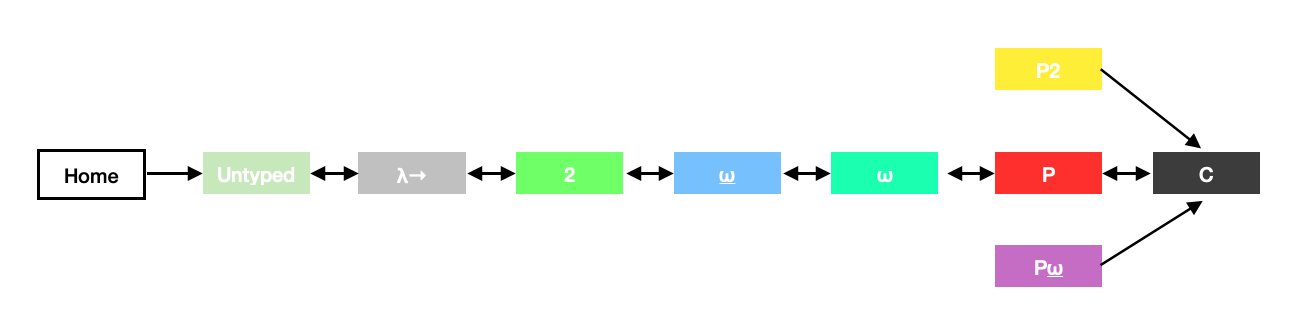
\includegraphics[width=1\linewidth]{dissertation/images/arrows_graph.png}
    \caption{A directed graph showing how the procession buttons moved the}
    \label{fig:enter-label}
\end{figure}    

Another fault I noticed during my observations was that most users only noticed the guide very late into their use of the website, despite admitting to needing help to understand some of the content.  Some users also found that there were things they did not understand, that were not explained in the guide.  In order to clarify these aspects of the website, I increased the size of the link which opens the guide, and added an explanation of sets and reduction notation.

While the constant movement of the cube was generally well received, some users also reported that the animation was distracting or slightly nauseating.  As a result I decided to add in an option to pause the cube's movement indefinitely.  This is achieved using a media query to search the computers settings to find if the user has 'reduced-motion' turned on, and using a port to set this value in the local library.  This value was then passed into the main function of my Elm program with the flags, where it could be changed with the press of a button.

One of the students who I surveyed was red-green colourblind, and as a result was less able to distinguish between the Polymorphic types and Dependent types.  In order to accommodate users with similar accessibility requirements, while keeping the same aesthetic that was liked by by the other users, I chose to implement a selectable colour blind mode.  This would be a button placed next to the reduced motion button which would toggle between the base state, using the same colours as before, and a mode which changes all of the colours to safe versions which can be more easily distinguished by users who are colourblind or otherwise visually impaired.

I then used the package 'HTML With context' to be able to check inside an Elm file if colourblind mode is set to normal or safe in the CSS variable.  I had to use CSS variables to do this, because to update the state in a similar way to how I had handled opening and closing the footer for instance, Color.elm would have to import files which depend on it, which is not allowed by the system.

The code I used for determining which background colour a div should use to use is shown here.  There were similar functions for text colour and border colour, as below.

\begin{lstlisting}[language = Elm]
colorForTheme : Theme -> Color -> String
colorForTheme theme color =
    case theme of
        Normal ->
            color.normal
        Colorblind ->
            color.safe

backgroundColor : Color -> Attribute msg
backgroundColor color =
    Html.WithContext.withContextAttribute
        (\{ theme } ->
            Attributes.style "background-color" (colorForTheme theme color)
        )
\end{lstlisting}

In `backgroundColor' you can see the lambda function inside the call to withContextAttribute which draws theme from the context, and passes it to `colorForTheme' which pattern matches the value to determine which version of the colour to use.

\begin{figure}[h!]
    \centering
    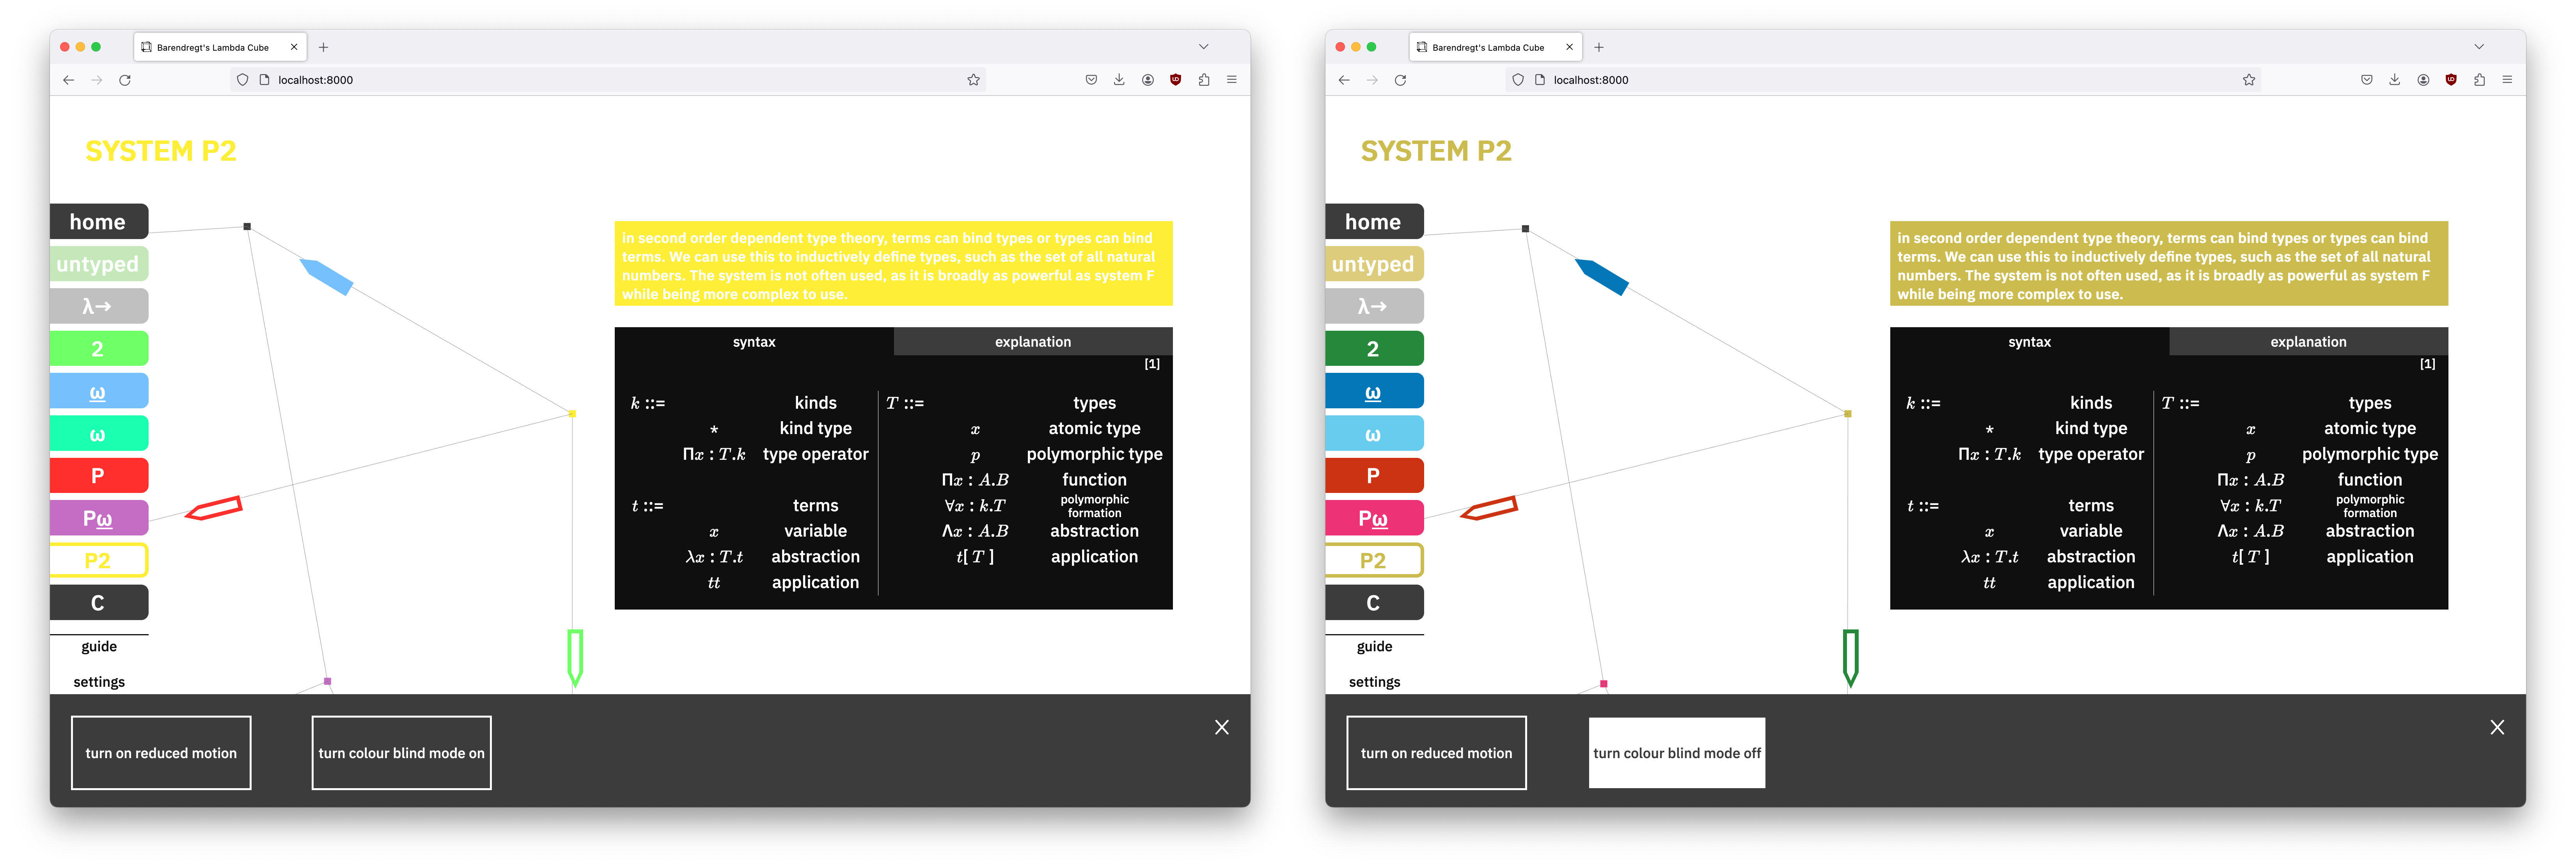
\includegraphics[width=1\linewidth]{dissertation/images/colourbind_collage.png}
    \caption{Screenshots comparing colourblind mode on and off}
    \label{fig:enter-label}
\end{figure}    

An advantage of this approach was that this solution is readily scalable.  By expanding the flags section, I could add further customisation features, such as an automatic night mode, with the same infrastructure with very little code.

\section{Conclusions}

My user studies were very useful for helping me find deficiencies in my website that I could not notice.  This was my main focus going into the studies, and I found the observation, conversation with the test taker and questionnaire worked very well at helping me to notice areas where I could improve my website.  By gathering multiple forms of feedback simultaneously, I believe that I was able to compensate for the small sample size to some degree.

The scores for the test sections of the study were universally quite low.  This could be because everyone surveyed had taken the programming languages course, which covers some of the necessary background, roughly a year ago, so had forgotten a lot of the relevant information.  It could also be that the user was not given long enough to explore the website, so were unable to learn enough to answer all of the questions.  A third reason for the poor test results could be that my website was generally ineffective at teaching the concepts that I wanted to express, however the scores were high enough and spread across multiple questions, so this reason does not seem likely, but should be considered.

The study was not useful in finding out whether my website was more effective than the other options, as I gathered no comparative data.  Although this was not the main aim of my studies, it would have been good to be able to prove that I had achieved the requirements set out earlier in the paper.

I should have instead split my study group into two sections, with one completing the same questions about the Wikipedia page I was using as a bench mark, and the other group to use my website.  By A/B testing the websites against each other, I would be able to draw statistically valid conclusions about the efficacy of my attempt to improve upon the previous projects discussed in the background.  This would be more effective than reusing the same group on both websites back to back, as it would mean that the users would be able to go into both experiences fresh, and the knowledge gained during the first trial would not effect their performance during their second one. 

However, this would effectively halve my sample size, which was already rather small due to the users having to have taken a specific course last year. This could result in any conclusions that I may have been able to draw not being statistically valid.

I do not believe that my website is currently accessible enough to users who rely on screen readers.  This is because some of the most important information is currently in MathML format which is less accessible than plain text.  There is also the problem of navigation, as although there are buttons such as the side bar or procession buttons arranged to take the user through an optimised route, this is not particularly clear to a student using a screen reader.  This problem with the main method of input the user has is very difficult to solve, as the main input modality, clicking on the nodes, requires sight.

%==================================================================================================================================
\chapter{Conclusion}    

\section{Summary}

I used Elm as the basis for my website, and WebGL to render a cube that could have its orientation and position changed in real time, so the user could effectively and seamlessly navigate to all eight corners. The website I created also had an explanation of the Untyped lambda calculus, as well as a guide on how to read the syntax necessary to understand the concepts contained at the nodes.

I used colour as a major design element, assigning a specific colour to each of the three type rules that are applied along the axes.  I did this to help build recognition of each type system, and to show the type systems mixing by mixing their constituent colours.

My main design problems were finding ways to display the information consistently, while still showing enough of the cube to keep a cohesive concept of it as the user moved between the nodes.  I ended up using a set of text boxes with specific styles, so that the user would recognise instantly where each different type of information would be stored.  As an example, a white text on a black background indicates that the text box is about the type system's syntax.

In order to depict the BNF syntax, I had to create a translator, using Deno, which takes a .tex file of an equation and returns a .elm file which can easily be rendered.  This allowed me to have much more granular control about how the syntax was depicted, as well as pre-render all of the content for a much faster uninterrupted user experience.

I focused my user studies on examining the user experience, gathering data about how likely they were to engage with different elements of the site during observation, and verifying how effective it was at teaching with a questionnaire.  Using the feedback I received, I was able to reorganise the page to make it more intuitive and accommodating to a wide range of users.

\section{Reflection}

I should have used a more structured timeline of granular tasks to be able to monitor my progress more closely, so that I could ensure that every part of my project received the appropriate amount of attention. 

Researching and finding sources proved to be one of the most difficult parts of the whole process.  There were many sources which referred to the same concept as other papers by a different name, and vague references to other works that I was unable to find.  This further convinced me of the need to have a strong citation system built into my website.  In retrospect, I should have done more of the research towards the start of the project, so that I could focus at one task at a time and not be constantly switching between coding and research.

I am very happy with my choice of Elm and the website I was able to create using it.  Its Model  View Update framework worked perfectly with the type of state machine style website that I had wanted to create.  Elm was also a good choice with its wider range of simple to install packages, which allowed me to prototype different solutions quickly.

I should have run different tests to validate my project, and struggled to find a suitable and large enough sample size to draw any statistically valid conclusions.  It also would have been helpful to have a longer observation period for each user, as it would let me make more notes and give them a longer time to explore the website and learn more, potentially making the quiz portion more valid.  

However I was able to utilise my user studies to find deficiencies in my project, and address them to make the website more effective and accessible.  It would have been better to test on only a group of people who were definitely familiar with lambda calculus, such as School of Computing Science staff or PhD students.  This would allow the users to spend less time learning the fundamentals, and focus on the content specific to the lambda cube.  This would be a smaller group, and one which is potentially harder to schedule to complete the studies, so it is perhaps not realistic to have only a trial group of users with a high level of background knowledge.

\section{Future Work}

I use inline style tags exclusively to control the look and layout of each element in the website.  This is a poor implementation, as it is very intensive to update every single necessary element when I decide to make a change, and leads to bloated and messy code full of repetition.  Midway through the project, I briefly considered using tailwind as an alternative to inline style tags, however decided that it was too great a change to reasonably make at that point in development. Tailwind is a CSS framework which would allow me to create a list CSS classes for each different element, streamlining my code and reducing the repetition significantly. 

Another idea which I had late into the project, and did not have time to implement, was an edit suggestion framework.  This would make the project collaborative by allowing anyone who visited the website to make suggestion or revision edits, which I or a future maintainer would be able to manually review and chose to implement or not.  This idea came to me while looking back through the Wikipedia article's version history.

The benefit of my proposed system over Wikipedia's system is that every edit is manually reviewed, so there is no chance of graffiti, and a much lower chance of incorrect information being mistakenly put onto the website as there is an extra step of review.  This system is feasible in my situation as there are vastly fewer possible places for edits to be made, and I am knowledgeable enough about the topic to be able to review each change, which is not an option for Wikipedia due to its scale.

The feature that I was most disappointed that I was not able to implement was screen reader accessibility on the sections of the page generated from .tex files.  These contain a large amount of the detailed information, which were less accessible to visually impaired users that I would have liked.  I am entirely unfamiliar with the use of screen readers, and with designing screen reader accessible websites, so was not able to add this feature in the limited development time.  In the future I would like to either add alternative text to all the currently inaccessible areas, or add some feature which automatically generates this content.

%==================================================================================================================================
%
% 
%==================================================================================================================================
%  APPENDICES  

\begin{appendices}

\chapter{Appendices}

\section{Task Sheet for User Evaluation}

\begin{figure}[h!]
    \centering
    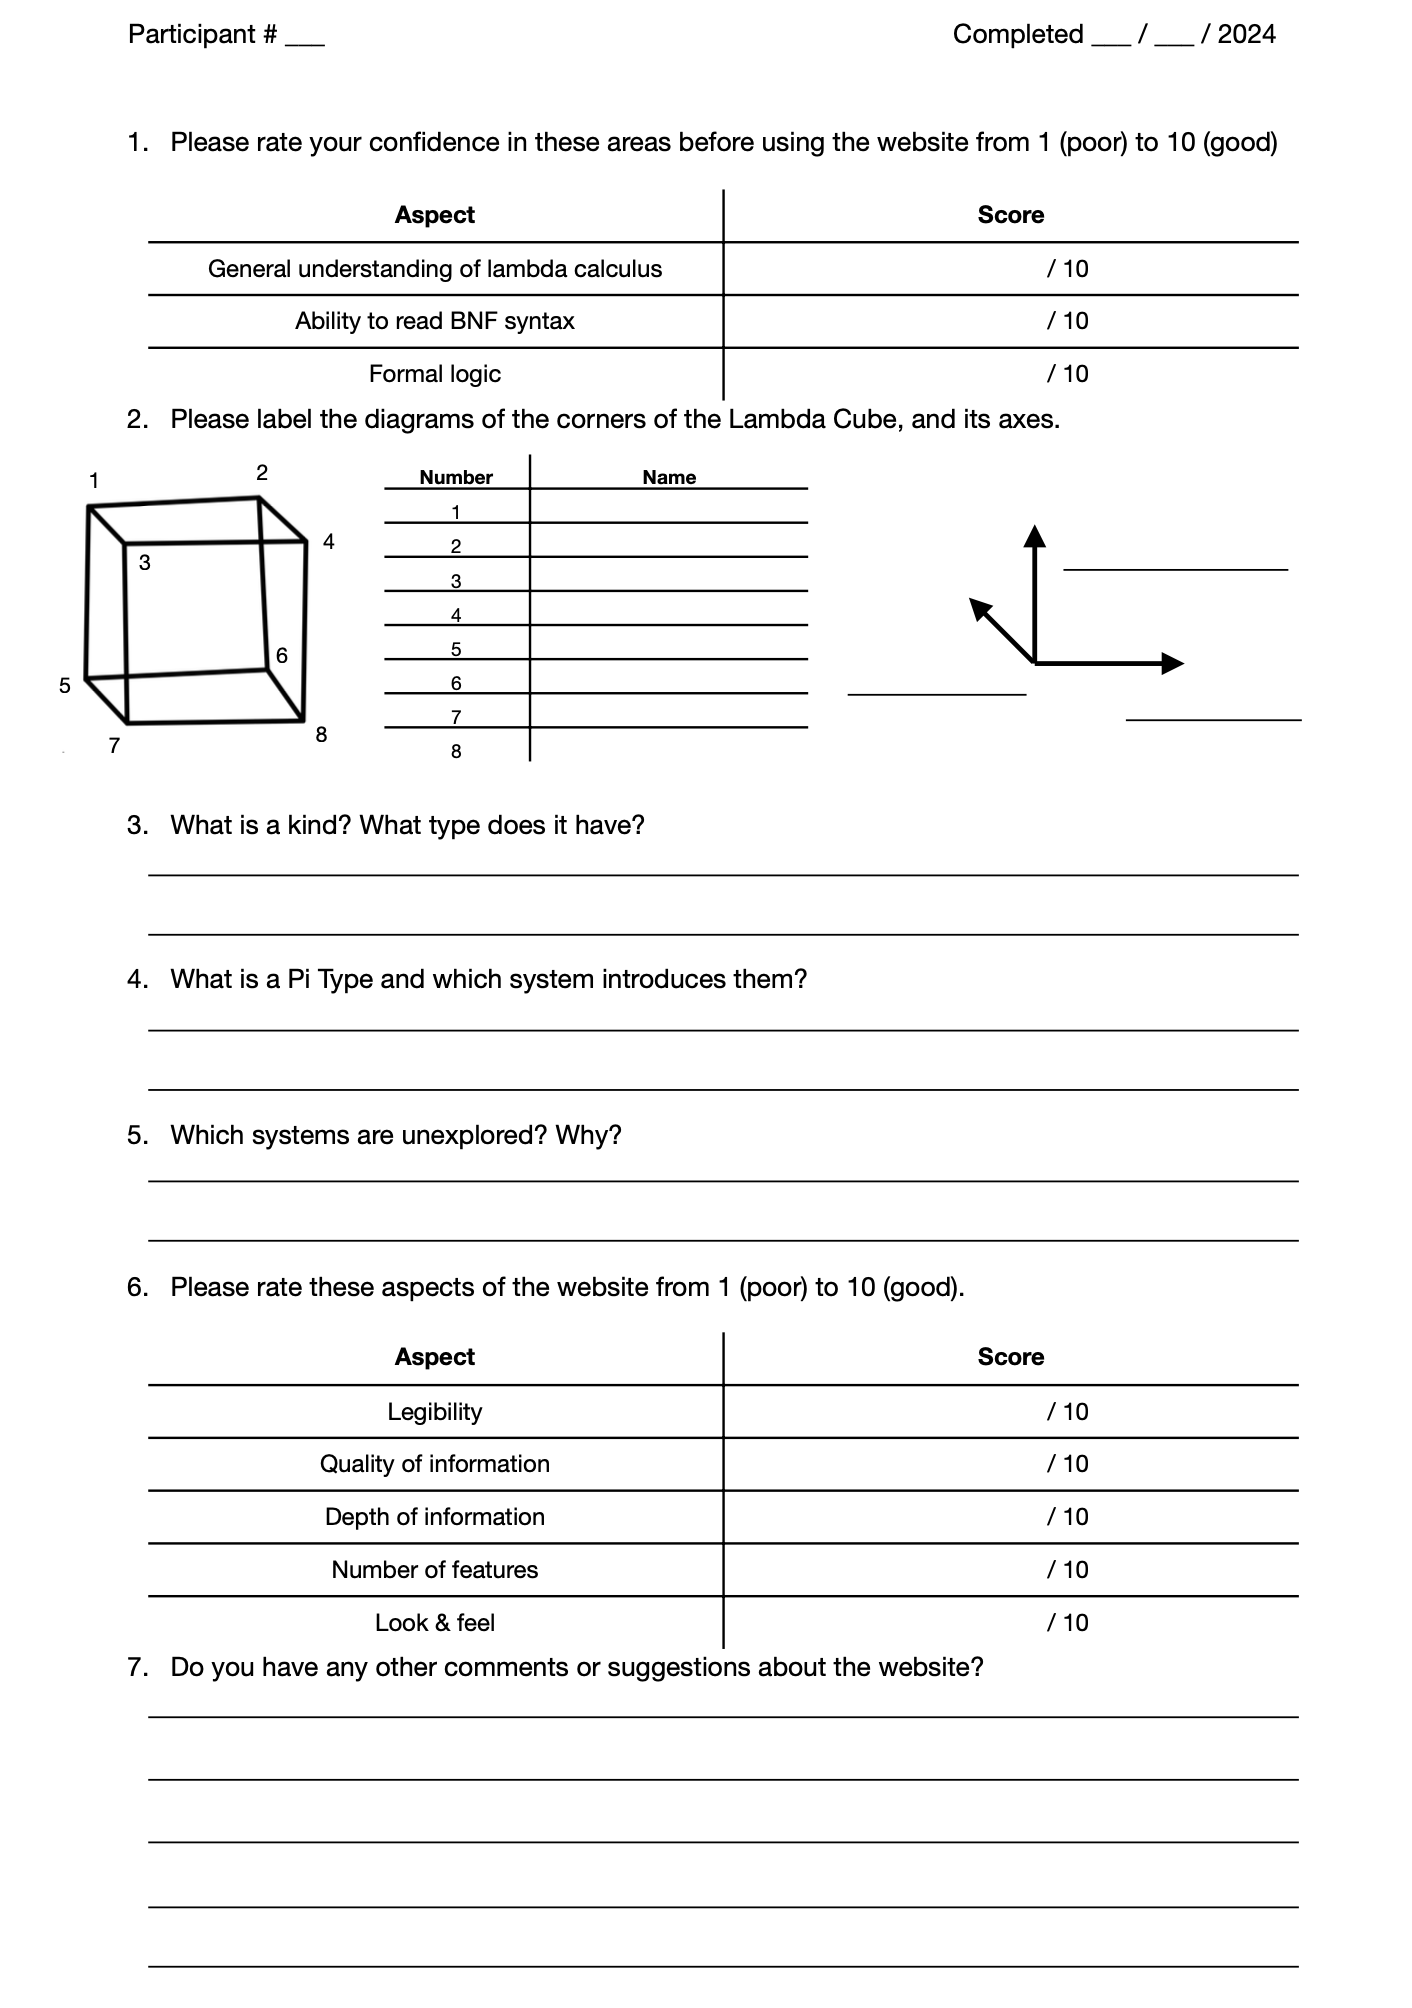
\includegraphics[width=0.8\linewidth]{dissertation/images/questions.png}
    \caption{A blank copy of the questionnaire used for user evaluation}
    \label{fig:enter-label}
\end{figure}

\end{appendices}

%==================================================================================================================================
% BIBLIOGRAPHY
% The bibliography style is abbrvnat
% The bibliography always appears last, after the appendices.
\bibliographystyle{abbrvnat}
\renewcommand{\thechapter}{0}
\bibliography{l4proj}
\end{document}
\bibliographystyle{abbrvnat}

\bibliography{l4proj}

\end{document}
